%==================================================================================================
%   LUKES THESIS TEMPLATE 1.2
%   -------------------------
%   This template is based upon the offcial IMM PhD Thesis template, it is enhanced with a number
%   of new features and a number of errors have fixed. This template is intended to be complied to
%   PDF using PDFLATEX and is tested using the MiKTeX 2.9 LaTeX distribution.
%   It is based on the official DTU-IMM Thesis template by Finn Kuno Christensen in 2009.
%   Small bugfixes by Kasper Laursen in 2012 and 2013.
%   -------------------------
%   Last Updated: 2012-09-19
%   Contact: lthhe@imm.dtu.dk
%==================================================================================================
%
%==================================================================================================
% DOCUMENT SETUP
%==================================================================================================
\documentclass[10pt,twoside]{book}                  %Official DTU-IMM Thesis document setup
%
%Set to 'print' for printed version, use 'net' for online version
\def\thesisversion{print}
%
%==================================================================================================
% PACKAGES
%==================================================================================================
\usepackage{LukeThesis}                             %Import Thesis base style
\usepackage{graphicx}
%\usepackage[utf8]{inputenc}
%\usepackage[T1]{fontenc}
%\usepackage{url}
\usepackage{hyperref}
\usepackage{pdfpages}
\usepackage{placeins}
\usepackage{graphicx}
\usepackage[font=small,labelfont=bf]{caption}
\usepackage{subfig}

%\usepackage{subcaption}
\usepackage{enumerate}
\usepackage{amsmath}
\usepackage{listings} %for showing program code
\usepackage{bm}
\usepackage{wrapfig}
\usepackage{lipsum}
\usepackage{float}
\usepackage{titlesec}	
\usepackage{amsfonts}
\usepackage{amssymb}
\usepackage[square,authoryear]{natbib}
\usepackage{epstopdf}
\usepackage{tabularx}
\usepackage{siunitx}
\usepackage{mathtools}
\usepackage{tcolorbox}
\usepackage{lscape}
\usepackage{multirow}

\tcbuselibrary{breakable}

\newtcolorbox{mybox}{colback=red!3!white,colframe=red!75!black,breakable,arc=0pt,outer arc=0pt}

\bibpunct{[}{]}{,}{a}{,}{,}
\raggedbottom 

%input{PhDMacros}                                   %Thesis specific macros
%
%==================================================================================================
% THESIS PROPERTIES (Modifiy these fields with your details)
%==================================================================================================
\def\thesisauthor{Alessandro Dal Corso}                     %Author
\def\thesistitle{Real-Time Rendering of Translucent Materials with Directional Subsurface Scattering}               %Title
\def\thesishandin{03-July}                       %Submission date (Day-Month}
\def\thesisdegree{M.Sc.}                              %Degree ('B.Eng', 'B.Sc.', 'M.Sc.' or 'PhD')
\def\thesisyear{2014}                               %Submission year
\def\thesisnumber{????}                             %DTU-IMM Serial number (do not include year)
\def\thesisISSN{0000-0000}                          %ISSN number
\def\thesiskeywords{subsurface,scattering,realtime,directional,dipole}  %PDF keywords
\derivethesisprops                                  %Derive dependent properties
%
%==================================================================================================
% SECTION NUMBERING SETUP
%==================================================================================================
\setcounter{tocdepth}{2}                            %2 adds sections up to subsections
\setcounter{secnumdepth}{3}                         %Subsubsections get a number when this is 3

\begin{document}
%------------------------
%Pre-frontmatter material
%------------------------
\prefrontmatter
%-------------------- 
%Frontmatter material
%--------------------
\frontmatter
\pagenumbering{roman}                               %Set frontmatter numbering style
\chapter{Abstract}

The goal of this thesis is to provide a fast rendering technique to render translucent materials. The goal is to create a method with low memory requirements that can be employed in real-time rendering applications such as computer games. To do this, we employ an analytical approach using a new BSSRDF model that includes the directionality of the incoming light into account. 

Our method incrementally builds the result over a certain number of frames, rendering the model from different directions and storing it in a texture, that then is sampled using shadow mapping in order to obtain the final rendering. The result is built by sampling other points on the surface using a special sampling pattern based on the optical properties of the material.

Using this approach, we obtained real-time results of 30 FPS for complex models of the magnitude normally employed in the computer game industry ($10^4$ triangles). The results are close in appearance to a path traced solution. Our method then provides a fast and robust way to account for the direction of the incoming light in the computation, providing a more realistic results that the ones reachable with previous analytical models.                                    %English summary of Thesis
%\markboth{}{}                                       %Set headings (left)(right)
%\input{tex/summaryDK.tex}                                   %Danish summary of Thesis
\markboth{}{}                                       %Set headings (left)(right)
\chapter{Preface}

\vspace{1cm}
This thesis was prepared at the DTU Compute department at the Technical University of Denmark in fulfillment of the
requirements for acquiring an M.Sc. in Digital Media Engineering.

The thesis deals with the efficient rendering of translucent materials, using and innovative model proposed by the author MSc thesis supervisor, Jeppe Revall Frisvad. Translucent materials consist of a particular class of materials like fruit, marble, skin, and other materials where the subsurface scattering effects cannot be neglected. 

The interest for real time rendering in the author arose during the course of his MSc in Digital Media Engineering, where he focused on the study line in Computer Games. For this study line, he had to take several courses in real time computer graphics, and from this courses he got his interest in advanced real time rendering techniques. In the spring 2014, professor Jeppe Revall Frisvad of DTU Compute proposed a research oriented thesis in creating a method for implementing the directional dipole in real time. The author deemed the topic to be a great opportunity to research in real time rendering techniques, and so he registered his application for this master thesis, \emph{\thesistitle}.

The thesis consists of a software implementation in C++, Qt and OpenGL and this report. The Qt framework used was taken from DTU course 02564, Real Time Graphics, and then greatly expanded in order to fit the needs of the thesis. All the code reported in this document was written by the author an does not come from the original framework. All the screenshots in this document were generated using the developed software, apart from all the path traced results, that were generated by Jeppe Revall Frisvad, and then sent to the author.

%==================================================================================================
% SIGNATURE AREA
%==================================================================================================
\begin{table}[ht]
\begin{tabularx}{\textwidth}{X}
\vspace{1.5cm}
Lyngby, \thesishandin-\thesisyear \\
\hfill \thesisauthor \\
\hfill \includegraphics[scale=0.4]{images/sig.png} \\
\end{tabularx}
\end{table}                                     %Preface
\markboth{}{}                                       %Set headings (left)(right)
\chapter{Acknowledgements}
I would like to thank my supervisor for this MSc project, Jeppe Revall Frisvad, for the constant support and help during the whole duration of this thesis. His constant help and meetings in his office, as well as his prompt replies to my e-mails, have been determinant in the development of this thesis. I would also like to thank professor Neils J\o rgen Christiansen for his suggestions and support during the weekly group meetings.

A special acknowledgment should be given to the T.I.M.E. double degree program, for giving me the opportunity to fulfill my dream of completing a Master Degree abroad. Without them, all my achievements in the past two years would not have been possible. From the University of Padua, I would like to thank professor Maria Elena Valcher, for helping with my study plan and all the bureaucracy a double degree program requires, and professor Emanuele Menegatti, for accepting on being my advisor for my MSc defense in Italy.

Finally, on a personal note, I would like to thank my family for the constant support they give to me, supporting also in my decision to study abroad. Of my friends, a special thank you is owed to my italo-colombian friend Marco Fraccaro for the help and the support in the last two years. I would also like to personally thank my colleague and Giacomo Baruzzo for in reading my thesis and giving suggestions on it. It is really impossible to list all the people that morally supported me during this master thesis, but I would like to thank them all for cheering me up during the most difficult moments of this thesis.                                %Acknowledgements
\markboth{}{} 
\clearpage
\thispagestyle{empty}
\begin{table}[ht]
\begin{tabularx}{\textwidth}{X}
\vspace{2cm}
\hfill \includegraphics[height = 6em]{images/jap.pdf} \\
\hfill \emph{Not seeing is a flower.} \\
\hfill (Japanese proverb) \\
\end{tabularx}
\end{table}
\markboth{}{}
%------------------
% Table of contents
%------------------
%\newpage\mbox{}\newpage
\chaptermark{Contents}
\pdfbookmark{\contentsname}{toc}
\renewcommand{\sectionmark}[1]{\markright{#1}}
\sectionmark{Contents}
\addtolength{\parskip}{-\baselineskip}
\tableofcontents
\addtolength{\parskip}{\baselineskip}
\renewcommand{\sectionmark}[1]{\markright{\thesection\ #1}}
%-------------
% Main content
%------------- 
\mainmatter
\definecolor{myblue}{HTML}{D4DEFF}
\definecolor{redcell}{HTML}{FFE8E8}
\definecolor{greencell}{HTML}{E8FFEB}
\definecolor{yellowcell}{HTML}{FFFDE8}
\newcommand{\vomega}{\vec{\omega}}
\newcommand{\x}{\mathbf{x}}
\newcommand{\cs}{C_{\phi}(\eta)}
\newcommand{\csinv}{C_{\phi}(1/\eta)}
\newcommand{\ce}{C_{\mathbf{E}}(\eta)}
\newcommand{\gl}[1]{\texttt{\nolinkurl{#1}}}
\newcommand\mycolor[1]{
\ifnum#1>100 \cellcolor{redcell}#1%
\else
\ifnum#1>60 \cellcolor{yellowcell}#1%
\else
\cellcolor{greencell}#1%
\fi
\fi
}
\newcolumntype{L}[1]{>{\raggedright\arraybackslash}p{#1}}
\newcolumntype{C}[1]{>{\centering\arraybackslash}p{#1}}
\newcolumntype{R}[1]{>{\raggedleft\arraybackslash}p{#1}}
\chapter{Introduction}
\label{chap:intro}
\emph{Subsurface scattering} (SS) is a physical phenomenon that naturally occurs in a wide range of natural materials. Some materials that exhibit a strong subsurface scattering effect in everyday life are milk, human skin and marble. Subsurface scattering occurs when light is partially absorbed by an medium, bounces repeatedly inside ("scatters") and finally exits the surface on another point of the material (as in Figure \ref{fig:ssdiagram}). The phenomenon that results is generally known as \emph{translucency}. We can see some examples of translucent objects in Figure \ref{fig:ex1}.

\section{Background}
Since the beginning of computer graphics, various attempts have been performed in order to model subsurface scattering. Some of these models involve Monte Carlo simulations of the light entering the medium \citep{Pharr:2000:MCE:344779.344824}, or other numerical techniques \cite{Fattal:2009:PMI:1477926.1477933,Kaplanyan:2010:CLP:1730804.1730821}. Other focus on approximating the diffusion of light within the material using an analytical approach, like \citep{Jensen:2001:PMS:383259.383319}.
 
\clearpage
\begin{figure}[!ht]
\centering
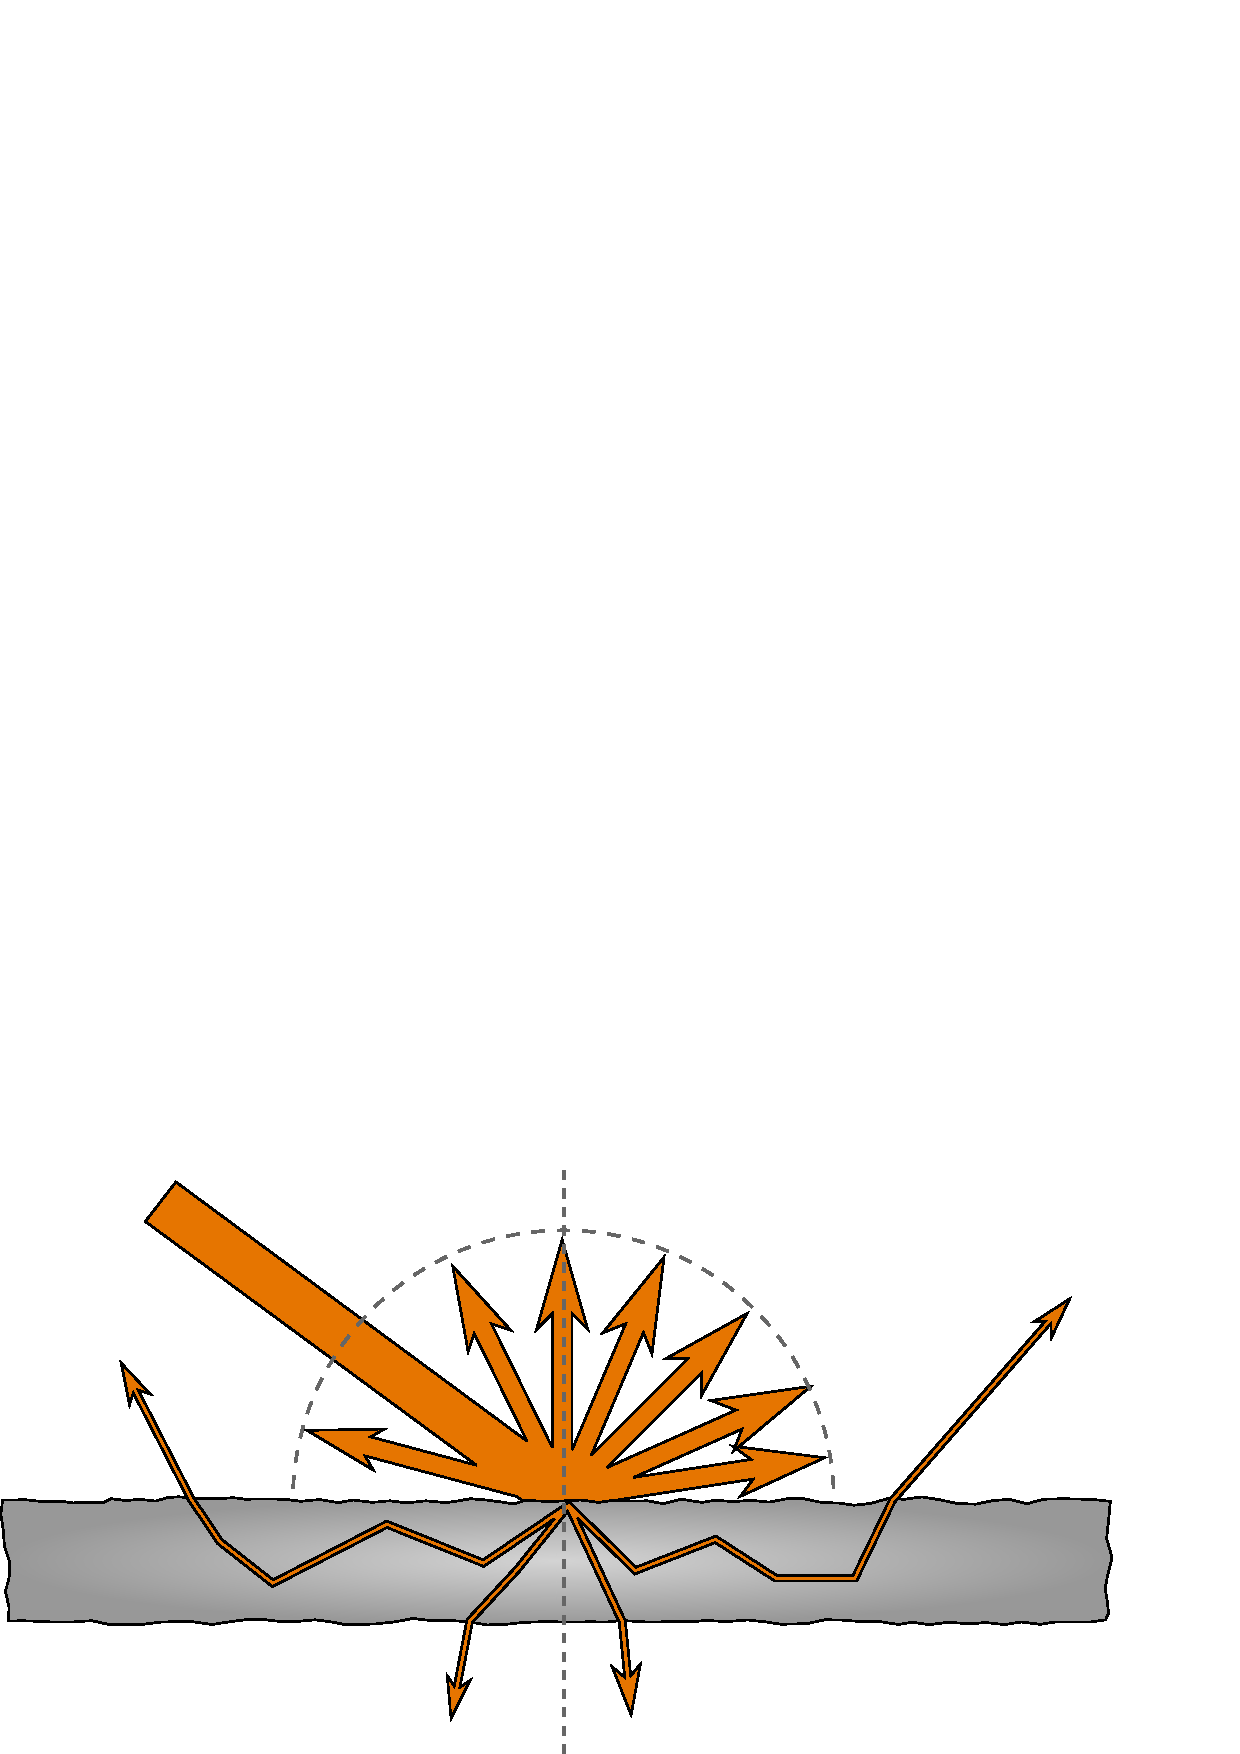
\includegraphics[width=0.8\textwidth]{images/diagram.pdf}
\caption{Diagram of subsurface scattering. Most of the incoming light gets reflected, but some of it enters the material and leaves it at a different point.}
\label{fig:ssdiagram}
\end{figure}

The first model that proposed and analytical approach was the one by \cite{Jensen:2001:PMS:383259.383319}, as an approximation of the radiative transfer equation. This approximation, called the \emph{diffusion approximation} \citep{books/daglib/0093591} has been exploited by different authors, in order to account for multi-layered materials \citep{Donner:2005:LDM:1186822.1073308}, heterogeneous materials \citep{journals/cgf/WangWHSYG10} and thin surfaces\citep{journals/cgf/WangWHSYG10}. A recent analytical approximation, proposed by \cite{IMM2013-06646}, extends the approximation in order to account for the directionality of the incoming light. All these analytical methods are based on BSSRDF models. A BSSRDF function is a functions that describes how light is transmitted between two points in a material, and is a generally dependent on the incoming light direction, the distance between the two points and the outgoing light direction.

In recent years, with the advent of programmable graphics cards (GPU), it has become possible to exploit these algorithms and bring them to interactive frame rates, and in some cases even to real time rendering. \cite{Jensen:2002:RHR:566654.566619} were the first to propose an efficient implementation for rendering subsurface scattering using an octree. More recently, several methods have been proposed, including image-based splats \citep{4736459}, sum-of-Gaussians filtering \citep{d'Eon:2007:ERH:2383847.2383869}, and grid-propagation based methods \citep{Borlum:2011:SSL:2018323.2018325}. We will introduce in detail some of these methods in Chapter \ref{chap:previous}, were we will review the existing literature in more detail.

\begin{figure}
\centering
\subfloat{
  \includegraphics[width= 0.9 \linewidth]{images/marble.jpg}
  \label{fig:ss1}
}
\\
\subfloat{
  \includegraphics[width= 0.9 \linewidth]{images/leaves.jpg}
  \label{fig:ss2}
} 
\\
\subfloat{
  \includegraphics[width=0.9 \linewidth]{images/candle.jpg}
  \label{fig:ss3}
} 
\caption{Some examples of translucent materials: marble, leaves and wax. The marble image and the candle are under the \href{http://creativecommons.org/licenses/by-sa/2.0/deed.en}{cc-by-sa} license, and are courtesy of Wikimedia Commons. The two images were cropped to fit the document. The leaves image was taken by Alberto Bedin and is used with permission.}
\label{fig:ex1}
\end{figure}

\section{Problem statement}

The goal of this thesis is to implement a real-time rendering technique in order to render directional subsurface scattering using the analytical model proposed by \cite{IMM2013-06646}. The technique should ideally obtain the same results as a path traced solution of the original model, but reducing the rendering times to a few milliseconds. To do this, we propose to employ the aid of the GPU programmable pipeline \citep{Fernando:2004:GGP:983868}. 

We found that there is a current gap in the knowledge on current real-time subsurface scattering techniques regarding the approach to directional models. In fact, most of the methods rely on the assumption that the BSSRDF function depends only on the distance between the entering and exiting point \cite{Jensen:2001:PMS:383259.383319}. This allows, for example, to pre-compute the BSSRDF function and use it in the computations, greatly increasing the performance \citep{4736459}. However, in the model proposed by \cite{IMM2013-06646}, this is not possible, as the direction of the incoming light must be taken into account. In fact, the model has too many degrees of freedom to make a pre-computation feasible. 

The model proposed by \cite{IMM2013-06646} offers a more realistic evaluation of subsurface scattering effects. A real-time working implementation would improve the quality of scattering materials in real-time graphics applications, such as real-time architectural visualization and computer games. In the latter field, in recent years there has been a renewed interest in real-time SS techniques, especially to model faithfully the appearance of skin on human faces. 

\section{Requirement analysis}

In this section, we will introduce some constraints and assumptions to limit the scope of our work. Some of these assumptions and constraints are well known to the graphics community, and they are generally introduced to allow better performance, quality and flexibility. Being a real-time rendering method implies that performance plays a big part in the decisions we have made in the process, but since the method uses a physically based approximation the final quality of the result is also important. In the process the aspect of flexibility has been taken into account, i.e. the capacity of the method to set the tradeoff between quality and performance. We will now list the assumptions we made in all the three described domains, quality, performance and flexibility. 

\subsection{Quality constraints}
 \label{sec:quality}
\begin{enumerate}
	\item Be visually close as much as possible to a path traced solution.
	\item Be consistent with the directional dipole model for a wide range of material properties. In particular, the method should perform well in the domain of quality where the directional dipole model excels (highly scattering materials).
	\item Be potentially able to render an object under an arbitrary number of different types of lights (point, directional, environment, etc.).
\end{enumerate}

\subsection{Flexibility requirements}	
\begin{enumerate}
	\item Work with the less amount as possible of provided model data, i.e. only the position data and eventually the normals should be provided in order for the method to run. In particular, no unwrap of the mesh (UV mapping) should be necessary. 
	\item Being able to be integrated in a game engine environment, using data from other computations (e.g. other lighting computations) and being adaptable to different lighting paths (forward and deferred shading).
  \item The quality versus performance tradeoff should be set by a potential artist or developer, with the fewest number of parameters as possible.
\end{enumerate}

\subsection{Performance requirements}

\begin{enumerate}
	\item Being real-time on a high-end modern GPU, i.e. one frame should take less that 100 ms (10 FPS) to render. The ideal result would be to reach a rendering time of less than 16 ms (60 FPS).
	\item Being as less dependent as possible from the geometrical complexity of the model.
	\item Being as less dependent as possible from the screen resolution.
	\item If the desired quality is not reachable within one frame, converge towards a result in a reasonable amount of time. Techniques should be used to approximate the required quality for the intermediate result. 
	\item Maintain a reasonable performance under changing light conditions, deformations and change of parameters, with little or none performance penalties.
	\item Employ the advantages of the directional dipole model to improve performance.
	\item Support up to a certain number of directional and point lights (up to 3 to 5 pixel lights, as in commercial engines\citep{unitymanual}).
	\item Require little or no pre-processing in order to be able to perform. If there is any pre-processing involved, it should be performed only at the beginning of the life cycle of the program. 
\end{enumerate}

%\section{Method overview}
%
%Our method consists of introducing the assumption that only the points within a certain radius from the point are contributing to the exiting light. Then, we take a certain number $N$ of these surface samples and compute their contribution to calculate the exiting light. The samples are distributed with an exponential distribution, in order to account more for the samples closest to the exiting point. The reader can get more details on the method in Chapter \ref{chap:method}. 

\section{Thesis Outline}

In this Chapter, we have given an introduction to the problem and stated the assumption that will guide us to the choices that we will make through our thesis. In Chapter \ref{chap:previous}, Related Work, we will describe in more detail some of the different approaches to subsurface scattering in literature. In Chapter \ref{chap:theory}, we will give a theoretical introduction to subsurface scattering and light transport theory, with a special focus on BSSRDF functions. In Chapter \ref{chap:method}, we will describe our method on approaching the problem on a theoretical basis. In Chapter \ref{chap:implementation} we will describe the actual implementation of the method, and the problems and limitations met during the process. In Chapter \ref{chap:results}, we will describe the tests we made and show the results, both in the domain of performance and quality, comparing them with the requirement analysis we made in the previous section. Then, we will describe some possible extensions to the method in Chapter \ref{chap:futurework}. We will wrap up everything in Chapter \ref{chap:conclusions}, where we will give our conclusions. 


\chapter{Related Work}
\label{chap:previous}
In rendering of subsurface scattering, most approaches rely on approximating correctly the \emph{Radiative Transfer Equation} (RTE). We identified two main approaches to the problem in literature:

\begin{description}
	\item[Analytical] One class of solutions consists of approximating the RTE or one of its approximations via an analytical model. These models can have different levels of complexity and computation times, and are often adaptable to a wide range of materials. However, often they rely on assumptions on the scattering parameters that limit their applicability.
	\item[Numerical] In this other class of solutions, a numerical approach is used instead of approximating the RTE with an analytical model. This methods include finite element methods and discrete ordinate methods, for which a numerical solution for the RTE is actually computed. While providing an exact solution, the computation times are longer. Other numerical approaches focus more on the appearance of the model and do not provide an exact solution for the RTE.
\end{description}

In this thesis, we focus on efficiently implementing a model that falls in the first category, the analytical models. In the following sections, we are going to describe approaches for each one of the mentioned categories, comparing them to our method.

\section{Analytical techniques}

In the analytical techniques, two different areas of research must be distinguished. The first area is the research on the actual models, while the second is research on how the actual models can be implemented efficiently. Each model is usually represented by a specific function called BSSRDF (\emph{Bidirectional Subsurface Scattering Reflectance Distribution Function}), that describes how light propagates between two points on the surface. An integration on the surface and all the directions must be performed in order to get how much light actually exits from a point on the surface. Implementation techniques focus on efficiently implementing this integration step, often making assumptions for which points the computation can be avoided. 

\subsection{Models}
Regarding the models, the first and most important is the dipole developed by \cite{Jensen:2001:PMS:383259.383319}. This models relies on an approximation of the RTE called the \emph{diffusion approximation}, which relies on the assumption of highly scattering materials. In this case, a BSSRDF for a planar surface in a semi-infinite medium can be obtained. The BSSRDF needs only the distance between two points to be calculated, and with some precautions can be also used with arbitrary geometry. This model does not include any single scattering term: it needs to be evaluated separately. The model has been further extended in order to account for thin object regions and multi-layered materials\citep{Donner:2005:LDM:1186822.1073308}.

A significant improvement of the model was later given by \cite{deondeon}, that improved the model to better fit path traced simulations without nearly any additional computation cost. A more advanced model based on quantization was proposed by \cite{D'Eon:2011:QMR:1964921.1964951}, that introduced a new physical foundation in order to improve the accuracy of the original diffusion approximation. Finally, some higher order approximation exist \citep{IMM2013-06646}, in order to account for the directionality of the incoming light and single scattering. This allows a more faithful representation of the model at the price of extended computation times. A comparison between the directional and the standard dipole can be seen in figure \ref{fig:comparison}.


\subsection{Implementations}

Most research on efficient implementations of a subsurface scattering analytical model has been made on the original model by \cite{Jensen:2001:PMS:383259.383319}. The first efficient implementation was proposed by \cite{Jensen:2002:RHR:566654.566619}, based on a two-pass hierarchical integration approach. Samples on the model are organized in an octree data structure, that then is used to render the object. In the first step, the radiance from the light is stored in the points. In the second pass, using the octree, the contribution from neighboring points is computed, clustering far points in order to speed up calculations. This approach can be adopted for the Jensen model, where the only parameter is the distance between the entering and exiting point. However, using the directional dipole, the samples cannot be clustered because of the directionality of the light: once we sum up the contribution from multiple lights, the contribution cannot be separated anymore. In fact, we would need a different clustering of the points for each light, that quickly becomes inefficient since whole octree would have to be stored on the GPU. 

\cite{Lensch:2002:IRT:826030.826632} approached the problem by subdividing the subsurface scattering contribution into two: a direct illumination part and a global illumination part (i.e. the light shining through the object). The global illumination part is pre-computed as vertex-to-vertex throughput and then summed to the direct illumination term in real-time. Compared to our method, this method requires a pre-computation step that depends on the geometry of the model, and thus deformation effects are not possible. Moreover, a coefficient has to be stored for each pair of vertex, that means a quadratic increase for increasing model size. Our method, on the other hand, occupies a memory space depending linearly on the number of vertices.

Translucent shadow maps \citep{Dachsbacher:2003:TSM:882404.882433} use an approach similar to standard shadow maps: they render the scene from the light point of view, and then calculate the dipole contribution in one point only from a selected set of points, according to a specified sampling pattern. As in \cite{Lensch:2002:IRT:826030.826632}, the contribution is split into global and local to permit faster computations. In our approach we will reuse some of the ideas introduced by translucent shadow maps: we will render the scene from the light point of view and we will reuse the information stored in the map such as depth, vertices and normals. However, our approach to using the values from the map is different from the original paper, as we will explain in chapter \ref{chap:method}. \cite{Mertens:2003:IRT:882404.882423} propose a fast technique based on radiosity hierarchical integration techniques, that unlike the previous implementation can handle deformable geometry.

Another important category of methods is screen space methods. \cite{1238246} propose an image space GPU technique that pre-computes a set of sample points for the area integration and then performs the integral over multiple GPU passes. \cite{d'Eon:2007:ERH:2383847.2383869,deonss} propose a method in image-space, interpreting subsurface scattering as a sum of images to which a gaussian filter has been applied. The gaussians are then summed with weights that make them fit the diffusion approximation. \cite{Jimenez:2009:SPR:1609967.1609970} improves further the technique, giving more precise results in case of skin. All these techniques assume that the diffusion profile can be pre-computed and then fitted with a sum of Gaussians: as we have already mentioned, this is not possible for the directional dipole, where the diffusion profile can change a lot depending on the angle of incidence of the incoming ray of light. Morevoer, even if we were able to compute the coefficients for each possible combination of parameters, it would not be possible to apply a gaussian filter with a different set of coefficients per point.

\cite{4736459} present a fast screen space technique that render the object as a series of splats, using GPU blending to sum over the various contributions. The diffusion profile in this case is pre-computed and stored as a texture. As in the previous techniques, the directionality of the incoming light does not allow the pre-computation of a diffusion profile. Moreover, the directional dipole is not symmetrical, so the splats would have to use a bigger radius in order to account for all the contribution, increasing computation costs.

\section{Numerical techniques}

Numerical techniques for subsurface scattering are often not specific, but come for free or as an extension of a global illumination numerical approximation, since the governing equations are essentially the same. Given their generality, they are usually slower than their analytical counterpart, and often rely on heavy pre-computation steps in order to achieve interactive framerates. The volumetric version of Jensen's Photon Mapping\citep{Jensen:1998:ESL:280814.280925} was originally developed to render participating media in general, but it has been adapted for subsurface scattering\citep{Dorsey:1999:MRW:311535.311560}. Classical approaches as a full Monte-Carlo simulation implementation of the light-material interaction, and finite-difference methods exist in literature\citep{raey}. 

Some less general methods have been introduced in order to devise more efficient approximations when it comes to the specific problem of subsurface scattering. \cite{raey} uses the diffusion approximation with the finite difference method on the object discretized on a 3D grid. \cite{Fattal:2009:PMI:1477926.1477933} uses as well a 3D grid, that is swept with a structure called light propagation map, that stores the intermediate results until the simulation is complete. All the numerical methods described so far are not real-time, and they are generally not feasible for a GPU environment. 

\cite{journals/cgf/WangWHSYG10}, instead of performing the simulation on a discretized 3D grid, makes the propagation directly in the mesh, converting it into a connected grid of tetrahedrons called \emph{QuadGraph}. This grid can be optimized to be GPU cache friendly, and provide a real-time rendering of deformable heterogeneous objects. The problem in this method is that the QuadGraph is slow to compute (20 minutes for very complex meshes) and has heavy memory requirements for the GPU. Compared to our method, this one requires an heavy pre-computation step, and allows only not-deformable objects. However, as most of propagation techniques, it can handle heterogeneous materials, while our method can not.

Precomputed radiance transfer methods are another class of general global illumination methods, that generally pre-compute part of the lighting and store it in tables\citep{Donner:2009:EBM:1531326.1531336}, allowing to retrieve it efficiently with an additional memory cost. The problem with this method compared to ours is that it requires a memory space that increases exponentially if we want to handle deformable materials and dynamic lighting. Moreover, it requires an heavy pre-computation in order to calculate the lighting coefficients. Our method, being analytical, does not required either a lot of memory or an hevay pre-computation step. 

A recent method called SSLPV - Subsurface Scattering Light Propagation Volumes \citep{Borlum:2011:SSL:2018323.2018325} extends a technique originally developed by \cite{Kaplanyan:2010:CLP:1730804.1730821} to propagate light efficiently in a scene using a set of discretized directions on a 3D grid. The method allows real-time execution times and deformable meshes with no added pre-computation step, with the drawback of not being physically accurate. Moreover, the required memory space on the GPU is larger than the one required than our method, since a voxelization of a mesh must be stored. 

Finally, for real-time critical applications (such as games), translucency is often estimated as a function of the thickness of the material, that is used to modify a lambertian term \citep{Tomaszewska2012,greenrtss}. A method by \cite{Kosaka:2012:RAR:2407156.2407206} uses an approach similar to the one we will describe in order to compute the thickness of the material using a different camera direction. While not physically accurate, this techniques allows to have a fast translucency effect that can be easily added to existing deferred pipelines. Compared to our method, this method requires no storage space and light computation. However, the risk is that the translucency effects are not represented faithfully, and some artifacts may appear, as pointed out in \cite{greenrtss}, and multisampling should be used in order to avoid artifacts. 

As we can see, in the reviewed literature so far there is not a proper way to account for direction in subsurface scattering in real-time. Given this literature review, we will introduce our method to handle directional subsurface scattering in real-time in chapter \ref{chap:method}. In the next chapter, we are going to give a theoretical introduction to a mathematical description of light transport, as well as giving the proper formulas and definition of the standard dipole model by \cite{Jensen:2001:PMS:383259.383319} and the directional dipole model presented by \cite{IMM2013-06646}.

\chapter{Theory}

In this chapter, we give a theoretical introduction to the topic dealt with in this thesis. The ultimate goal of this chapter is to introduce and describe a analytical model for subsurface scattering. First, we will give a brief introduction to what light is, and how we physically describe it. Secondly, we will introduce the basic radiometric quantities that will be used throughout the chapter. Then, we will describe how this quantities are related and can be used to describe light-material interaction, using reflectance functions, of which BSSRDF functions are a special case. Finally, we will introduce subsurface scattering and the diffusion approximation, concluding with a description of two BSSRDF functions actually used to describe it, by \cite{Jensen:2001:PMS:383259.383319} and \cite{IMM2013-06646}.

\section{Light and Radiometry}
Light is a form of electromagnetic radiation, that propagates through space as a sinusoidal wave. Usually by "light` we usually refer to \emph{visible light}, the small part of the electromagnetic spectrum the human eye is sensible to (see Figure \ref{fig:spectrum}). This small window is between the \SI{380}{\nano\meter} of the infrared and \SI{750}{\nano\meter} of the ultraviolet, but the precise boundaries vary according to the environment and the observer. Instead explicitly noted, we will use the terms light and visible light interchangeably in this report.

The study of light is usually referred as optics. In computer aided image synthesis, we are interested in representing faithfully how visible light propagates though the scene and how interacts with materials. In addition, we are usually interested on lighting effects that are noticeable at human scales (\SI{1}{\milli\meter} - \SI{1}{\kilo\meter}). For example, we are interested in subsurface scattering, absorption and emission phenomena but not in diffraction, interference and quantum effects, that for visible light happen on a microscopic scale (\SI{1}{\nano\meter} - \SI{1}{\micro\meter}). 

\begin{figure}[!ht]
\centering
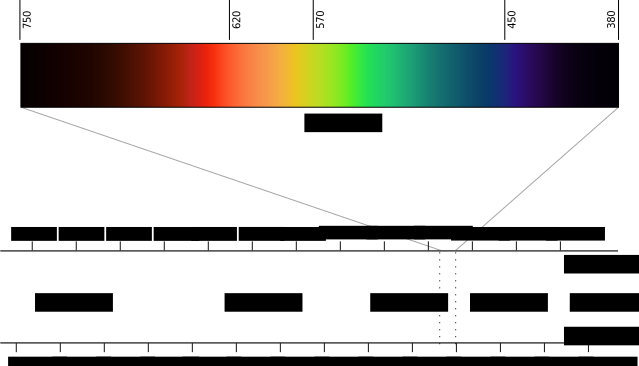
\includegraphics[width=1.0\textwidth]{images/spectrum.pdf}
\caption{The electromagnetic spectrum.}
\label{fig:spectrum}
\end{figure}

The study of the measurement of electromagnetic radiation is called \emph{radiometry}. The energy of light, like all the others forms of energy, is measured in \emph{Joules} [\si{\joule} $=$ \si{\kg\meter\square\per\second\square}], and its power in \emph{Watts} [\si{\watt} $=$ \si{\kg\meter\square\per\second\cubed}]. \emph{Photometry}, on the other hand, measures electromagnetic radiation as it is perceived from the human eye, and limits itself only to the visible spectrum, while radiometry spans all of it. The quantities for energy and power are called respectively \emph{talbot} [\si{\candela\second}] and \emph{candela} [\si{\candela}]. 

In image synthesis radiometry is employed, as its quantities directly derive from the electromagnetic theories, are universal, and can be easily converted to the photometric ones when necessary. The most important radiometric quantities used in computer graphics are \emph{radiant flux}, \emph{radiant energy}, \emph{radiance}, \emph{irradiance} and \emph{intensity}.

\section{Radiometric quantities}

\subsection{Radiant flux}
The radiant flux, also known as radiant power, is the most basic quantity in radiometry. It is usually indicated with the letter $\Phi$ and it is measured in joules per seconds [\si{\joule\per\second}] or Watts [\si{\watt}]. The quantity indicates how much power the light irradiates per unit time. Given its nature, the radiant flux is independent from the distance from the light source.

\subsection{Radiant energy}
Radiant energy, usually indicated as $Q$, is the energy that the light carries in a certain amount of time. Like all the other SI units for energy, it is measured in joules [\si{\joule}]. Radiant energy is usually obtained integrating the radiant flux along time for an interval $\Delta T$:

$$
Q = \int_{\Delta T} \Phi \; dt
$$

Due to the dual nature of the light, the energy carried by the light can be derived both considering the flux of photons as particles, or considering light as a wave. We will not dig further into the topic, because for rendering purposes is not important if we characterize light as a flux of particles or as a sinusoidal wave.

\subsection{Irradiance}

Irradiance, usually defined as $E$, is the radiometric unit that measures the radiant flux per unit area \emph{falling} on a surface. It is measured in Watts per square meter [\si{\watt\per\meter\square}]. It is obtained by further deriving the radiant flux by the area:

$$
E = \frac{d\Phi}{dA}
$$

Irradiance is usually the term in literature used for the \emph{incoming} power per unit area. The converse, i.e. the irradiance leaving a surface, it is usually referred as \emph{radiant exitance} or \emph{radiosity}, and indicated with the letter $B$.
 
\subsection{Intensity}
Intensity is defined as the differential radiant flux per differential solid angle:

$$
I(\vec{\omega}) = \frac{d \Phi}{d \omega}
$$

It is measured in Watts / steradian [\si{\watt\per\steradian}] and it is indicated with the letter $I$. Intensity is often a misused term in the physics community, as it is used for many different measures. Depending on the community, intensity may refer to irradiance or even to radiance (see the following section). We will refer to intensity as it is generally interpreted by the optics community, i.e. radiant intensity. 

\subsection{Radiance}
Radiance is the most important quantity in image synthesis. It is defined precisely as the differential of the flux per solid angle per projected surface area, and it is measured in Watt per steradian per square meter [\si{\watt\per\steradian\meter\square}].

$$
L(\vec{\omega}) = \frac{d^2 \Phi}{d\omega dA \cos \theta}
$$

Where $\theta$ is the angle between the surface normal and the incoming ray of light (so that $\cos\theta = \vec{n} \cdot \vec{\omega}_i$). Radiance is important in image synthesis because it is the natural quantity to associate with a ray of light, as it remains constant along it. In addition, the sensibility of the human eye to light is directly proportional to the radiance. For a discussion on why radiance is related to the sensitivity of sensors and the human eye, see X.

All the other radiometric quantities can be derived from radiance:

\begin{equation}
\begin{split}
E &= \int_{2\pi} L_i(\vec{\omega}) \cos\theta \; d\omega \\
B &= \int_{2\pi} L_o(\vec{\omega}) \cos\theta \; d\omega \\
I(\vec{\omega}) &= \int_A L(\vec{\omega}) \cos\theta \; dA \\
\Phi &= \int_A \int_{2\pi} L(\vec{\omega}) \cos\theta \; d\omega dA
\end{split}
\label{eq:radiancederivation} 
\end{equation}

For simplicity of notation, in the previous notations the dependence from the point of incidence $\mathbf{x}$ has been dropped. In principle, all the quantities listed in equation \ref{eq:radiancederivation} are dependent on $\mathbf{x}$.

\subsection{Radiometric quantities for simple lights}

To help with the formulas used later in the report, we derive the above mentioned radiometric quantities for the two simplest types of light, i.e. directional and point lights.
\begin{itemize}
	\item \textit{Directional lights} simulate very distant light sources, in which all the rays of light are parallel (e.g. the sun). They are represented by a direction $\vec{\omega}_l$ and a constant radiance value, $L$. 
	\item \textit{Point lights} simulate lights closer to the observer. Isotropic point lights are represented by a position of the light $\mathbf{x}_l$ and a constant intensity $I$. Point lights have a falloff that depends on the inverse square law, i.e. the radiance diminishes with the square of the distance.
\end{itemize}

Table \ref{table:radio} shows different radiometric quantities evaluated for point and directional lights, for a surface point $\mathbf{x}$ with surface normal $\vec{n}$. 

\renewcommand{\arraystretch}{1.8}
\begin{table}[!ht]
    \centering
    \begin{tabularx}{0.95\textwidth}{|X|X|X|}
    \hline
    Quantity   & Directional light & Point light \\ \hline
    Cosine term       & $\cos\theta = \vec{n} \cdot \vec{\omega}_l$ & $\cos\theta = \frac{(\mathbf{x} - \mathbf{x}_l) \cdot \vec{n}}{|\mathbf{x} - \mathbf{x}_l|}$     \\ \hline

    $\Phi(\mathbf{x})$ Flux       & $\infty$                  & $4 \pi I$           \\ \hline
    $E(\mathbf{x})$ Irradiance & $L \cos\theta $                 & $I \frac{\cos\theta}{|\mathbf{x}_l - \mathbf{x}|^2}$          \\ \hline
    $I(\mathbf{x},\vec{\omega})$ Intensity  & $\infty$                 & $I$           \\ \hline
    $L(\mathbf{x},\vec{\omega})$ Radiance   & $L$               & $\frac{I}{|\mathbf{x}_l - \mathbf{x}|^2}$           \\ \hline
    \end{tabularx}
\caption{Different radiometric values for simple light sources. Note that flux and irradiance for a directional light are infinite because they are integrated over an infinite area.}
\label{table:radio}
\end{table}

\section{Reflectance Functions}
 
After introducing the basic radiometric quantities, we still lack a way to describe light material interaction. More precisely, we need a way to relate the incoming and the outgoing radiance on a point of a chosen surface. As we have already discussed before, we use radiance since is the radiometric quantity that is directly proportional to what the human eye measures. 

\subsection{BRDF functions}

One of the possible way to describe light-material interaction is by using a BDRF function, acronym for \emph{Bidirectional Reflectance Distribution Function}. The BRDF function $f(\mathbf{x}, \vec{\omega}_i, \vec{\omega}_o)$ is defined on one point $\mathbf{x}$ of the surface as the differential ratio between the exiting radiance and the incoming irradiance:

\begin{equation}
f(\mathbf{x}, \vec{\omega}_i, \vec{\omega}_o) = \frac{d L_o(\mathbf{x}, \vec{\omega}_o)}{d E_i(\mathbf{x}, \vec{\omega}_i)} = \frac{d L_o(\mathbf{x}, \vec{\omega}_o)}{L_i(\mathbf{x}, \vec{\omega}_i) \cos\theta_i d \vec{\omega}_i}
\label{eq:brdf}
\end{equation}

The BRDF states that the incoming and the outgoing radiance are proportional, so that the energy hitting the material at the point $\mathbf{x}$ is proportional to the energy coming out from the point. The BRDF function is generically reciprocal for the Hemholtz reciprocity principle ( $f(\mathbf{x}, \vec{\omega}_i, \vec{\omega}_o) = f(\mathbf{x}, \vec{\omega}_o, \vec{\omega}_i)$), and anisotropic (if the surface changes orientation and $\vec{\omega}_i$ and $\vec{\omega}_o$ stays the same, the resulting BRDFs are different). In addition, it is positive( $f(\mathbf{x}, \vec{\omega}_o, \vec{\omega}_i) \ge 0$), and conserves energy, so that the energy of the outgoing ray is no grater that the one of the incoming one ($\int_{2\pi}  f(\mathbf{x}, \vec{\omega}_o, \vec{\omega}_i) \cos\theta_o d\vec{\omega}_o \le 1$).

By inverting equation \ref{eq:brdf}, we obtain the so-called \emph{reflectance equation}:

$$
L_o(\mathbf{x}, \vec{\omega}_o) = \int_{2\pi} f(\mathbf{x}, \vec{\omega}_i, \vec{\omega}_o) L_i(\mathbf{x}, \vec{\omega}_i) \cos\theta_i d\vec{\omega}_i
$$

That later we will extend to obtain the rendering equation. The BRDF function has some limitations, being not able to account for all phenomena. For example, with a BRDF it is not possible to account for subsurface scattering phenomena, because it assumes the light enters and leaves the material in the same point. To model these phenomena, more complicated functions are needed, like the BSSRDF function described later in this chapter. 

\subsection{Examples of BRDF functions}

There are many examples of BRDF functions in literature. In this section, we will introduce three of the simplest ones: for a more exhaustive description of BRDF functions, refer to X. The three BRDFs are the lambertian or diffuse BRDF, the specular or mirror BRDF and the family of glossy BRDFs.

\subsubsection{Lambertian BRDF}

In the lambertian BRDF, the incoming radiance is distributed equally in all directions, regardless of the incoming direction. To do this, the BRDF must be constant:

$$
f(\mathbf{x}, \vec{\omega}_i, \vec{\omega}_o) = k_d
$$

We can check that then the radiance is scattered equally in all directions by simple integration:

\begin{equation*}
\begin{split}
L_o(\mathbf{x}, \vec{\omega}_o) &= \int_{2\pi} f_d L_i(\mathbf{x}, \vec{\omega}_i) \cos\theta_i d\vec{\omega}_i \\
L_o(\mathbf{x}, \vec{\omega}_o) &= k_d \int_{2\pi} L_i(\mathbf{x}, \vec{\omega}_i) \cos\theta_i d\vec{\omega}_i \\
L_o(\mathbf{x}, \vec{\omega}_o) &= k_d \; E(\mathbf{x}) \\
\end{split}
\end{equation*}

The lambertian model is an ideal model, so very few material exhibit a lambertian diffusion, like unfinished wood or spectralon, a synthetic material created in order to have a lambertian diffusion. 

\subsubsection{Mirror BRDF}

Another simple kind of BRDF is the perfectly specular BRDF, or mirror BRDF. In this function, all the incoming radiance from one direction $\vec{\omega}_i$ is completely diffused into the reflected direction $\vec{\omega}_r$, defined as $\vec{\omega}_r = \vec{\omega}_i - 2 (\vec{\omega}_i \cdot \vec{n}) \vec{n}$. The resulting BRDF is defined as follows:

$$
f(\mathbf{x}, \vec{\omega}_i, \vec{\omega}_o) = \frac{\delta(\vec{\omega}_o - \vec{\omega}_r)}{\cos\theta_i} 
$$

The function $\delta(\vec{\omega})$ is a hemispheric delta function. Once integrated over a hemisphere, the function evaluates to one only for the vector $\vec{\omega} = \mathbf{0}$. Putting the BRDF into the reflectance equation gives the following outgoing radiance:

\begin{equation*}
L_o(\mathbf{x}, \vec{\omega}_o) = \begin{cases}
L_i(\mathbf{x}, \vec{\omega}_i)  &\text{if $\vec{\omega}_o = \vec{\omega}_r$}\\
0 &\text{otherwise}
\end{cases}
\end{equation*}

that is the expected result, as all the radiance is reflected into the direction $\vec{\omega}_r$.

\subsubsection{Glossy BRDFs}

As we can see from real life experience, rarely objects are completely diffuse or completely specular. These two models are idealized models, that represent an ideal case. So, to create a realistic BRDF model, we often need to combine the two terms and add an additional one, called glossy reflection. This term is often needed to model the behavior of the surface more realistically, especially at grazing angles.

The most used BRDF model used to model glossy reflections is based on microfacet theory. In this theory, the surface of an object is modeled as composed of small mirrors. In one of its classical formulation, the BRDF is represented as:

$$
f(\mathbf{x}, \vec{\omega}_i, \vec{\omega}_o) = \frac{D G R}{4 \cos\theta_r \cos\theta_i} = \frac{G R}{4} \frac{(\vec{n}\cdot\vec{h})^s}{(\vec{n}\cdot\vec{r})(\vec{n}\cdot\vec{\omega}_i)}
$$

$D$ regulates how microfacets are distributed, and it is often modeled as $(\vec{n}\cdot\vec{h})^s$, where $\vec{h}$ is the half vector between the eye and the light, and $s$ is an attenuation parameter. $\vec{h}$ is defined as:

$$
\vec{h} = \frac{\vec{\omega}_o + \vec{\omega}_i}{\left\| \vec{\omega}_o + \vec{\omega}_i \right\|}
$$

$G$ accounts for the object self shadowing, while $R$ is the Fresnel reflection term (more details in section Y).	$\vec{r}$ is the reflection vector as defined in the previous section. See figure Z on how the vectors for the glossy reflection - $\vec{n}$, $\vec{h}$ and $\vec{r}$ - are defined.

Various alternative definitions exist for the $D$ and $G$ function, varying among the literature. Other glossy models not based on microfacet theory do exist as well. 

\subsection{The rendering equation}

Given the reflectance equation, it is possible to generalize it in order to model all the lighting in an environment. In fact, this form of the reflectance equation does not account for two important factors. 

The first factor are emissive surfaces. We need to add an emissive radiance term $L_e(\mathbf{x}, \vec{\omega})$ that models how much radiance is a point on a surface emitting in a certain directions. This is useful to model lights as any other surface in the scene. Note that point lights have a singularity: they emit infinite radiance on the point they are placed.

The second factor is that the reflectance equation accounts only for direct illumination. In general, we want to model global illumination, i.e. to include also light that bounced onto another surface before reaching the current surface. To model this, we can replace the $L_i$ term in the reflectance equation with another term $L_r$ that accounts for reflected radiance. This term can be usually modeled as the product of the radiance of the light plus a visibility function $V(\mathbf{x})$.

Accounting for all the described factors, we reach one formulation of the rendering equation:

$$
L_o(\mathbf{x}, \vec{\omega}_o) = L_e(\mathbf{x}, \vec{\omega}) + \int_{2\pi} f(\mathbf{x}, \vec{\omega}_i, \vec{\omega}_o) L_i(\mathbf{x}, \vec{\omega}_i) V(\mathbf{x}) \cos\theta_i d\vec{\omega}_i
$$

This form of the rendering equation is still not completely general, since it is based on a BRDF, so it is not possible to model subsurface scattering effects or wavelength-changing effects (like iridescence). We will extend the rendering equation in order to account for these phenomena later on in this chapter.

\subsection{Fresnel equations}

Until now, on the described BRDF models, we did consider only the reflected part of the radiance. When a beam of light coming from direction $\vec{\omega}_i$ hits a surface, only part of the incoming radiance gets reflected, while another part gets refracted into the material. As we can see from the setup from figure Z, we obtain the two vectors $\vec{\omega}_r$ and $\vec{\omega}_t$, the reflected and refracted vector, defined as follows:

\begin{equation*}
\begin{split}
\vec{\omega}_r &= \vec{\omega}_i - 2 (\vec{\omega}_i \cdot \vec{n}) \vec{n} \\
\vec{\omega}_t &= \eta ((\vec{\omega}_i \cdot \vec{n}) \vec{n} - \vec{\omega}_i) - \vec{n} \sqrt{1 - \eta^2 (1 - (\vec{\omega}_i \cdot \vec{n}) ^ 2)}
\end{split}
\end{equation*}

Where $\eta = \frac{n_1}{n_2}$ is the relative index of refraction of the material. With this setup, we can use a solution to Maxwell's equations for wave propagation to describe how light spreads between reflected and refracted directions. What we obtain are called \emph{Fresnel coefficients}. The coefficients are different according to the polarization of the incoming light, so there are two for the reflection ($R_s$, $R_p$) and two for transmission ($T_s$, $T_p$). The coefficients relate the incoming and outgoing power of the light, and by differentiation, the radiance as well.

\begin{equation*}
\begin{split}
R_s = \left|\frac{n_1 \cdot \cos\theta_i - n_2 \cdot \cos\theta_t} {n_1 \cdot \cos\theta_i + n_2 \cdot \cos\theta_t}\right|^2 \;\;\;&\;\;\; R_p = \left|\frac{n_1 \cdot \cos\theta_t - n_2 \cdot \cos\theta_i} {n_1 \cdot \cos\theta_t + n_2 \cdot \cos\theta_i}\right|^2\\
T_s = \frac{n_2 \cdot \cos\theta_t}{n_1 \cdot \cos\theta_i} \left|\frac{2 n_1 \cdot \cos\theta_i}{n_1 \cdot \cos\theta_i + n_2 \cdot \cos\theta_t}\right|^2 \;\;\;&\;\;\; T_p = \frac{n_2 \cdot \cos\theta_t}{n_1 \cdot \cos\theta_i}  \left|\frac{2 n_1 \cdot \cos\theta_i}{n_1 \cdot \cos\theta_t + n_2 \cdot \cos\theta_i}\right|^2
\end{split}
\end{equation*}


In most computer graphics applications (and this is reasonable for most of the real-world lights), we assume that the two polarizations are equally mixed. So, we will use the coefficient $R = \frac{R_s + R_p}{2}$ and $T = \frac{T_s + T_p}{2}$ in our calculations. Note that $R + T = 1$, so the overall energy is conserved.

\section{Light transport and subsurface scattering}
\subsection{BSSRDF functions and generalized rendering equation}

In order to be able to model subsurface scattering 

\subsection{Scattering parameters}
 emission, absorption, scattering and phase functions
\subsection{Standard dipole model}
\subsection{Directional dipole model}

\chapter{Method}
In this chapter, the goal is to solve the problem that we have presented, i.e. rendering translucent materials efficiently using the directional dipole. First of all, we will start this chapter with a list of constraints and assumptions that we will use to devise our method. Secondly, we will give a theoretical justification of our method, deriving a discretization of the rendering equation that can be actually implemented in a GPU environment. Then, we will discuss some possible sampling patterns and how they could possibly improve the results of the final rendering. Then, we will introduce how the actual scattering parameters are acquired in an experimental environment, in order to obtain a plausible result. 

%Finally, we will introduce a method to extend our result to enviromnent ligthins, using a particular sampling pdf.

\section{Constraints and assumptions}

\section{Method overview}

\section{Sampling patterns}

\section{Parameter acquisition}
When rendering translucent materials, it is important that we have the right scattering properties, in order to match the appearance of real world objects. The scattering parameters may be tweaked by the artist and set up manually, but this is a long process since the the scattering properties are not directly related to material appearance. In order to avoid this problems, the scattering parameters are measured from samples taken from real world objects. In this section, we will give an overview of two methods used to estimate the scattering parameters.

The first method was presented alongside the standard dipole model by \cite{Jensen:2001:PMS:383259.383319}. The measurement apparatus consists of a series of lenses that focus the light on the sample. The light power $\Phi$ is measured by calibrating the sensor with a spectralon sample. A picture of the sample is then acquired at different exposure, in order to build an high dynamic range image. This is necessary since the scattering decays exponentially, so a high range is needed to have meaningful measurements. The measured data are then fitted to diffusion theory in order to obtain the scattering coefficients. Due to the nature of the measurement, it is not possible to measure the mean cosine $g$ of the material, but only the reduced scattering coefficient $\sigma_s' = \sigma_s (1 - g)$ and the absorption coefficient $\sigma_a$. This measurement model uses the diffusion approximation to work, so it shares the same limitations: it is valid only for materials where $\sigma_a \ll \sigma_s$.

The second method, proposed by \cite{Narasimhan:2006:ASP:1141911.1141986} proposes a method to measure the scattering coefficient by dilution. The assumption is that water does not interfere with the scattering properties of the materials dissolved within it for small distances (less than \SI{50}{cm}). Naturally, the material needs then to be already in  a liquid form, or to be a powder that can be easily dissolved in water. The setup of the experiment is a box full of water with a camera and an area light. High dynamic range picture of the material dissolved in water are then taken, and the scattering coefficients can be measured with a low error. Various measurements at different concentrations are needed in order to get an effective measurement of the coefficients, but then the coefficients can be extrapolated for any concentration. 

Some of the scattering properties measured thanks to this method are reported in table \ref{table:scatteringcoefficients}. This coefficients will be used throughout the report when referencing to a specific material.
\clearpage
\begin{landscape}
\renewcommand{\arraystretch}{1.8}
\begin{table}[!ht]
    \centering
    \begin{tabular}{|l|ccc|ccc|ccc|c|c|}
    \hline
    \multirow{2}{*}{Material}               & \multicolumn{3}{|c|}{Absorption, $\sigma_a$}     & \multicolumn{3}{|c|}{Scattering, $\sigma_s$}     & \multicolumn{3}{|c|}{Mean cosine, $g$}    & \multirow{2}{*}{$\eta$} & \multirow{2}{*}{Source} \\ \hline
               &R& G      & B     & R & G      & B      & R   & G     & B     &  &  \\ \hline
    {Apple}                  & 0.0030 & 0.0034 & 0.0046 & 2.29   & 2.39   & 1.97   & -     & -     & -     & 1.3    & J      \\
    {Ketchup}                & 0.061  & 0.97   & 1.45   & 0.18   & 0.07   & 0.03   & -     & -     & -     & 1.3    & J      \\
    {Marble}                 & 0.0021 & 0.0041 & 0.0071 & 2.19   & 2.62   & 3.00   & -     & -     & -     & 1.5    & J      \\
    {Potato}                 & 0.0024 & 0.0090 & 0.12   & 0.68   & 0.70   & 0.55   & -     & -     & -     & 1.3    & J      \\
   { Whole milk}             & 0.0011 & 0.0024 & 0.014  & 2.55   & 3.21   & 3.77   & -     & -     & -     & 1.3    & J      \\
    {Coffee}                 & 0.1669 & 0.2287 & 0.3078 & 0.2707 & 0.2828 & 0.297  & 0.907 & 0.896 & 0.88  & 1.3    & N    \\
    {Soy milk}               & 0.0001 & 0.0005 & 0.0034 & 0.2433 & 0.2714 & 0.4563 & 0.873 & 0.858 & 0.832 & 1.3    & N      \\
    {Wine (merlot)   }       & 0.7586 & 1.6429 & 1.9196 & 0.0053 & 0      & 0      & 0.974 & 0     & 0     & 1.3    & N      \\
    {Beer (Budweiser)}       & 0.1449 & 0.3141 & 0.7286 & 0.0037 & 0.0069 & 0.0074 & 0.917 & 0.956 & 0.982 & 1.3    & N      \\
    {White grapefruit juice} & 0.0096 & 0.0131 & 0.0395 & 0.3513 & 0.3669 & 0.5237 & 0.548 & 0.545 & 0.565 & 1.3    & N      \\ \hline
    \end{tabular}
		\caption{Scattering material parameters estimated using different methods. For the source field, \texttt{J} materials come from \cite{Jensen:2001:PMS:383259.383319}, while \texttt{N} materials come from \cite{Narasimhan:2006:ASP:1141911.1141986}. Note that the materials measured with the technique proposed in \cite{Jensen:2001:PMS:383259.383319} are without the $g$ coefficient.}
		\label{table:scatteringcoefficients}
\end{table}
\end{landscape}
\clearpage
%\section{Environment lights}

%Stuff to insert:
%\begin{itemize}
%	\item Generation of random points (details)
%	\item Noise generation on GPU (caveats)
%	\item Sampling patterns (details)
%	\item Layered rendering (details)
%	\item Shadow mapping (for lights) (details)
%	\item Ping-ponging and accumulation (details)
%	\item Texture Views and mipmap generation (memory optimization) (caveats)
%	\item Engine structure (no)
%	\item Extension: compute shaders
%	\item Extension: image load store (meh)
%	\item Extension: subroutines (meh)
%	\item Sampling colormap
%	\item Alternative: voxelization
%	\item Multiple lights
%	\item Different types of light
%	\item Skyboxes
%\end{itemize}


%Caveats:
%\begin{itemize}
%	\item Oversampling issues in final combinaiton (multisampling of depth map)
%	\item Combination delta
%	\item Shadow bias
%  \item Random rotation
	
%\end{itemize}

\chapter{Implementation}

In this chapter, we will introduce the implementation details of our method. The difference between this chapter and the previous one is that the concepts introduced in the method chapter are easily adaptable to any kind of implementation environment, while in this chapter we focus on a GPU-oriented implementation. First, we will give a general outline of our algorithm. Then, we will take each one of the single parts of the algorithm and discuss them separately. After introducing the details of the algorithm, we will discuss some caveats that are necessary in order to eliminate defects and artifacts in our algorithm. Finally, we will discuss our implementation, introducing some possible implementation alternatives in order to compare them in the result section.

\section{Environment}

In order to better contextualize some of the choices and the code parts that will be introduced in this section, we will first introduced the environment used in our implementation. The method we are going to discuss was made using the OpenGL API, version 4.3 (released in August 2012), a multi-platform API used for rendering 2D and 3D accelerated graphics. With the OpenGL API comes together GLSL, the OpenGL Shading Language, used for writing pieces of code to be run on the GPU, called \emph{shaders}. Our method uses some advanced features of OpenGL 4.3, so it is not immediately portable to previous generation hardware, and runs only on high-end modern GPUs. On the CPU side, we use an extended framework based on Qt, a C++ library that allows to create OpenGL contexts and graphical interfaces in an easy way.

In this chapter, we describe the implementation details of our technique, using the approximation of the rendering equation introduced in the previous chapter. We start by giving a rather generic introduction of our algorithm, introducing then all the implementation details. 


%\section{Requirements}
%
%Our algorithm, in order to be generic and applicable to a wide range of situations must meet some requirements. 
%
%
%\begin{itemize}
  %\item The algorithm should be \emph{accurate}, so that the renderings are as close as possible to reference images generated using a offline Monte-Carlo simulation. 
	%\item The algorithm should be \emph{fast}, executing at interactive frame rates.
	%\item The algorithm should be \emph{uv-independent}, not relying on a pre-made UV mapping of the object in order to being able to perform. The algorithm should work only if basic geometric features are provided (vertices and normals).
	%\item The algorithm should be \emph{adaptable}, handling in real-time dynamic light changes and object deformations. So it will not possible to use light baking or geometry form factors.
%\end{itemize}
%
%If it is not possible to satisfy all the previous within the strict constraints of real-time rendering, we want to create an algorithm that gets as close as possible to the requested result. The algorithm should progressively progressively improve and converge to an accurate result whenever possible (e.g. when the light in the scene is not changing).

\section{Algorithm overview}

By keeping the limitations presented in the previous chapter in mind TODO, we introduce our four pass algorithm. The algorithm is inspired by \emph{translucent shadow maps} TODO, that we presented in chapter TODO. The general idea is to first render the scene from the light point of view, then place the disk we discussed in the method chapter TODO directly on the generated texture. We use many directions in order to capture all the sides of the object. In this section, we will assume to only have one directional light $L_d$, $\vomega_d$ and one not-deformable object in the scene. We will discuss later how to extend the method to multiple light sources.

\textbf{Step 1 - Light buffer} \\

In the first step, positions and normals of the object are rendered into a texture from the light point of view. As in standard shadow mapping we create and store a matrix to convert between world space and texture light space. Depth testing in this step is enabled.

\begin{figure}[!ht]
\centering
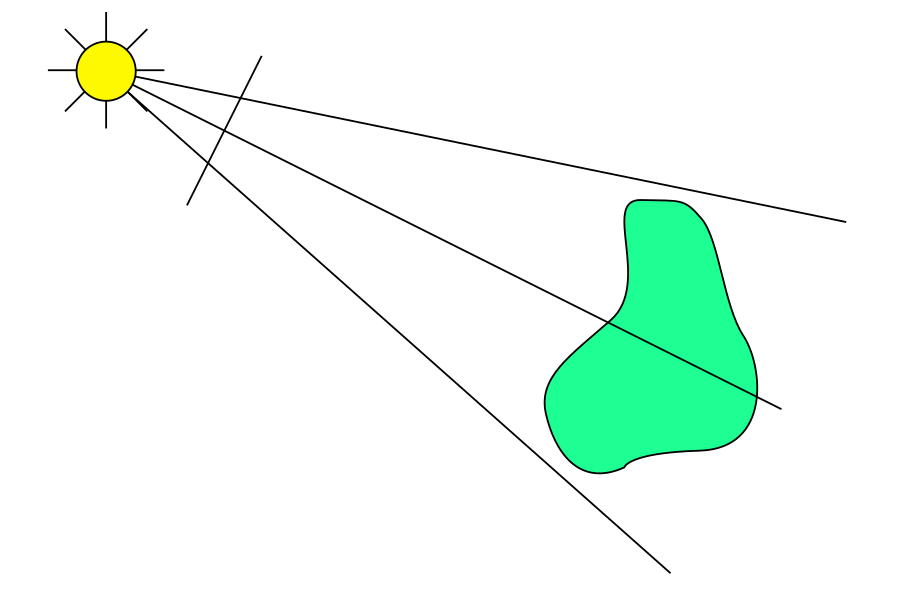
\includegraphics[width=0.8 \linewidth]{images/method/step1.pdf}
\caption{Render to G-buffer. Note that the frustum and the light direction are aligned.}
\label{fig:step1}
\end{figure} 


\begin{figure}
\centering
\subfloat[{Vertex buffer}]{
  \includegraphics[width=0.5 \linewidth]{images/method/vertices.png}
  \label{fig:vbuff}
}
\subfloat[{Normal buffer}]{
  \includegraphics[width=0.5 \linewidth]{images/method/normals.png}
  \label{fig:nbuff}
} 
\label{fig:lightbuffers}
\caption{State of the vertex and normal buffer after rendering from a directional light. The model used was the Stanford bunny from the Standford 3D Scanning repository.}
\end{figure}

\FloatBarrier

\textbf{Step 2 - Render to radiance map} \\
In the second step, we render the object from $K$ different directions into a radiance map. The radiance map is organized as a layered texture, where each layer represents a direction. The points on which to place the cameras are chosen randomly. On each layer, we accumulate the result over different frames. On the rendering step, for each pixel that corresponds to an exitance point $\x_o$ the shader samples $N$ points from the texture rendered in the previous step. If the sampled point is valid, it is then used to calculate the BSSRDF and accumulate it in the resulting radiance map. So, this step calculates the following:

$$
R^{t,k}(\x_o) = L_d \sum_{i = 1}^N S(\x^{t,k}_i, \vomega^t_l, \x_o, \vomega_o) \exp\left(\sigma_{tr} r^{t,k}_i\right), \ \ t \in [0,T], \ \ k \in [0,K-1] 
\label{eq:evolution_step}
$$

\begin{figure}[!ht]
\centering
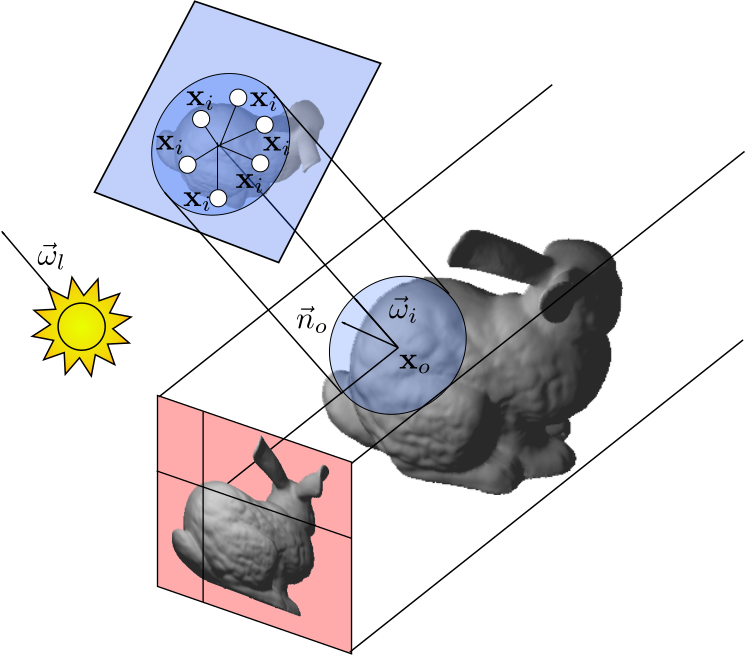
\includegraphics[width=0.9 \linewidth]{images/method/step2_improved.pdf}
\caption{Render to the radiance map. When we render the point $\x_o$, the position in the lightmap is calculated and the values $\x_i$ in the samples are calculated and summed over.}
\label{fig:step2}
\end{figure} 

Where we recall that we have introduced an exponential term in order to compensate for the exponential displacement of the sampling pattern. We introduced also a time $t$ parameter, that represents the fact that the result change over time, and a $k$ parameter, that represents the current direction we are rendering to. We can see how we are rendering a point from one of the considered directions in Figure \ref{fig:stepfrustum}. Also in this case, the texture space - world space conversion matrices are stored and prepared to be reused in the final combination step. 

We can appreciate that rendering the light from the camera point of view comes with two important advantages:

\begin{itemize}
	\item If the disk is placed in texture space, it is automatically oriented towards the light direction, that is $\vomega_d = \vomega_l$.
	\item The light renders in the texture only the points directly visible from it, that are also the points where the light radiance is maximum. In addition, if we sample the lightmap on any point, we get the corresponding vertex that is closest to the light.
\end{itemize}

This two factors allows us to sample the most optimal point and direction in where to place the disk, as we described it in section TODO.
 
\begin{figure}[!ht]
\centering
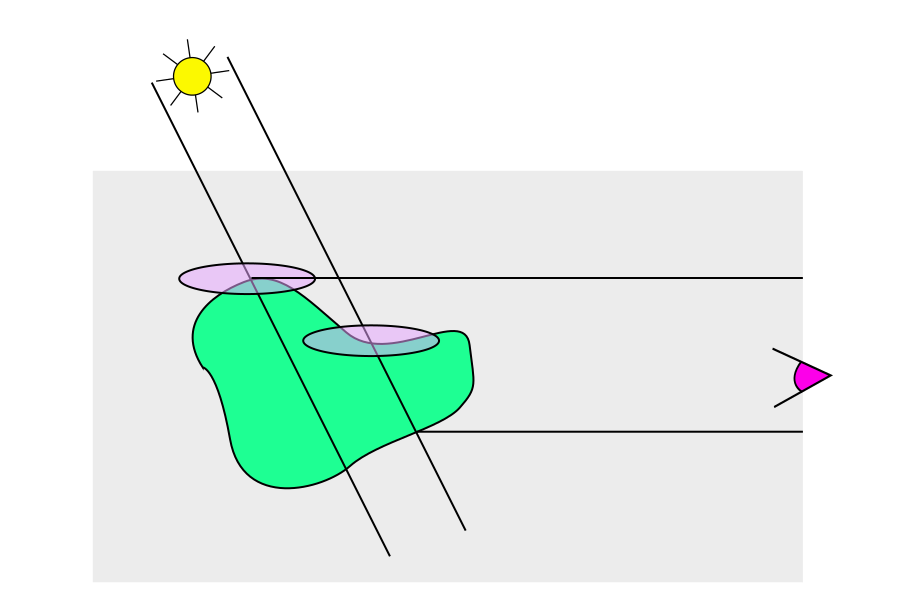
\includegraphics[width=\linewidth]{images/method/step2}
\caption{Render to cubemap, side view. The gray area represents the frustum of the current direction's camera (orthographic). We have three different cases of a point on the surface: $\x_o^1$ is visible from both the light and the camera, so the disk is placed on it. $\x_o^2$ is visible from the camera but not from the light, so the disk is placed in the closest position to the light. $\x_o^3$ is not visible from the camera, so it is discarded.}
\label{fig:stepfrustum}
\end{figure} 

In this step, there is an accumulation process going on:

$$
\tilde{R}^{t,k} = \sum_{i = 0}^{t-1} R^{i,k} + R^{t,k} = \tilde{R}^{t-1, k} + R^{t,k}
$$

$\tilde{R}$ here represents the actual value that is stored in the texture or loaded from the previous one. We need an accumulation process in order to deal with the fact that the result from the previous computation are not reaching a satisfying result within one frame, so they need to be accumulated over a period of $T$ frames in order to reach converge to an appreciable result. In order to do this, the sampled points need to change on different frames (see section TODO) for more details. 

Naturally, the accumulation process works only if the scene does not change. A change can be a relative change of positions between the points on the model and the light, so if the model gets rotated or scaled (translation for directional lights is irrelevant), the accumulated result has to be discarded and the accumulation started all over. The cameras are locked with the model, so the pixels are always aligned irregardless of the model matrix of the object. This is why in equation \ref{eq:evolution_step} the dependence from time of the point $\x_o$ and $\vomega_o$ have been dropped. Obviously, the dependence must be reintroduced in case we are dealing with deformable objects.
 
\textbf{Step 3 - Combination} \\
In this step, we have the final render of our model. While all the previous steps were not rendering anything in the scene (making a render-to-texture), in this scene we do an actual rendering of the model. Using the matrices prepared in the previous step, for each fragment on the surface we sample all the layers in the texture as illustrated in Figure \ref{fig:step3}. In order to do this, we need also to sample the depth map generated in the previous step. We can define this sampling as a visibility function to test if a point $\x$ belongs to layer $k$:

$$
V^k(\x) = \begin{cases}
1 & \text{if $\x$ is visible from the $k$th camera} \\
0 & \text{otherwise}
\end{cases}
$$
Given this function, we can simply represent the outgoing radiance by simply averaging the summation over the $K$ layers:

$$
L_{SS}^t(\mathbf{x}) = \frac{A_c}{N (t + 1)} \frac{\displaystyle\sum_{k = 0}^{K-1}V^k(\x) \tilde{R}^{t,k}(\mathbf{x})}{\displaystyle\sum_{k = 0}^{K-1}V^k(\x)}
$$

The first factor $\frac{1}{t + 1}$ is to average over the number of frames, while the second is the average area of a sample in the circle $\frac{A_c}{N}$, that is necessary to complete the equation as described in TODO. We note that we tried to move all the layer-independent computation into the final computation step, in order to save as much performance as possible. 

\begin{figure}[!ht]
\centering
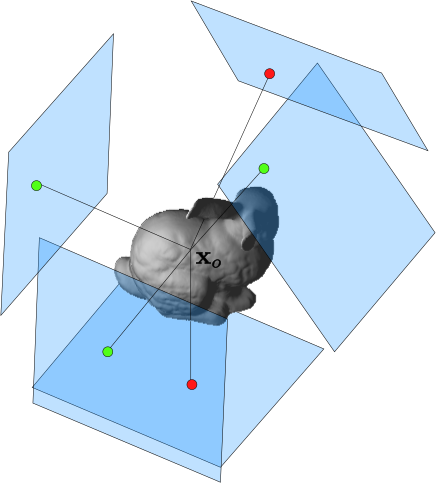
\includegraphics[width=0.6 \linewidth]{images/method/combination.pdf}
\caption{Final combination step. The blue quads indicates each one of the radiance map layers, as seen from their direction. We can see that in the point $\x_o$ the contribution from three faces (green dots) is considered. For the remaining two faces (red dots), the contribution is not considered as the point is not visible.}
\label{fig:step3}
\end{figure} 

We are not done yet, as for now we have computed the radiance only deriving from subsurface scattering. For finally describing the illumination of our scene, we need also to include a factor based on the surface reflection. Since the subsurface scattering radiance is already multiplied by a transmittance Fresnel term (in the BSSRDF equation in TODO) $T(\eta,\vomega_o)$ we the reflection color multiplied by the converse transmission term $1 - T(\eta,\vomega_o)$:

$$
L^t(\x, \vomega_o) = L_{SS}^t(\x) + (1 - T(\eta,\vomega_o)) L_i(\x, \vomega_o - 2 (\vomega_o \cdot \vec{n}) \vec{n})
$$

$L_i$ can be the radiance coming from other objects or by an environment map. After this, we just need to perform gamma correction in order to get the final result. Given the gamma coefficient $\gamma$, we perform gamma correction by:

$$
L_{gamma}^t(\x, \vomega_o, \gamma) = L^t(\x,\vomega_o)^{\frac{1}{\gamma}}
$$

And we can finally send the radiance to the output device.

\section{Implementation details}
In this section, we will further expand the overview  given in the previous section adding further details. We organized this section in topics, rather than following the order given by the algorithm, since most of the topic we will introduce will be used in multiple places. We will point out where each topic will be used in the algorithm.

\subsection{Render-to-texture}
In a graphics API, and more specifically in OpenGL, all the output from a final shader stage is usually sent to the display device in order to be displayed on the screen. However, it is possible to redirect the output into another memory area of the GPU and reuse it for further computations. This allows to create complicated rendering techniques such as the ones described in this report. 

In OpenGL, is possible to redirect the output more specifically to a texture object. We can do this through a so-called \emph{framebuffer object} (FBO). A FBO is a complex collection of objects that allow offscreen rendering. A FBO has \emph{attachment points}, to which we can attach textures between the various things. A texture can be attached to one of the output color channels of the fragment shader (\gl{GL_COLOR_ATTACHMENT0}, \gl{GL_COLOR_ATTACHMENT1}, ...), to the depth buffer output (\gl{GL_DEPTH_ATTACHMENT}) or to the stencil buffer output (\gl{GL_STENCIL_ATTACHMENT}).

The connection between the framebuffer and the texture can be set in a initialization step. Afterwards, by simply binding the FBO we will render to the configured texture:

\begin{lstlisting}[language=C++,label=lst:rendertotextureinit,caption={Render to texture example, initilalization phase. Note the call to \gl{glFramebufferTexture2D}}]
GLuint tex,fbo;
// Generating texture
glGenTextures(1, &tex);
glBindTexture(GL_TEXTURE_2D, tex);
[...] // setting up texture parameters...
glTexImage2D(GL_TEXTURE_2D, 0, GL_RGBA16F, size, size, 0, GL_RGBA, GL_FLOAT, 0);


glGenFramebuffers(1,&fbo);

// connecting current fbo and texture
glBindFramebuffer(GL_DRAW_FRAMEBUFFER, fbo);
glFramebufferTexture2D(GL_DRAW_FRAMEBUFFER, GL_COLOR_ATTACHMENT0, GL_TEXTURE_2D, tex, 0);
glBindFramebuffer(GL_DRAW_FRAMEBUFFER, 0); //Binding back main framebuffer
\end{lstlisting}

\begin{lstlisting}[language=C++,label=lst:rendertotexturerender,caption={Render to texture example, rendering phase. Since we have not configured and FBO for depth and stencil buffers, depth testing and stencil should be disabled at this point.}]
glBindFramebuffer(GL_DRAW_FRAMEBUFFER, fbo);
GLenum buffers[] = {GL_COLOR_ATTACHMENT0};
glDrawBuffers(1, buffers);
[...] // draw model
\end{lstlisting}

\subsection{Layered rendering}
Layered rendering is a special feature used to render to a special type of texture called \emph{layered texture}. Let us take as an example the step 2 of our algorithm, where we need to render the object from $K$ different directions. A first approach to this would be to create $K$ 2D textures of type \gl{GL_TEXTURE_2D}, and perform $K$ draw calls, rebinding the texture on the current FBO each time. OpenGL, however, provides a way to do this faster, and with a single draw call, potentially reducing the rendering costs due to context switching.

\begin{figure}[!ht]
\centering
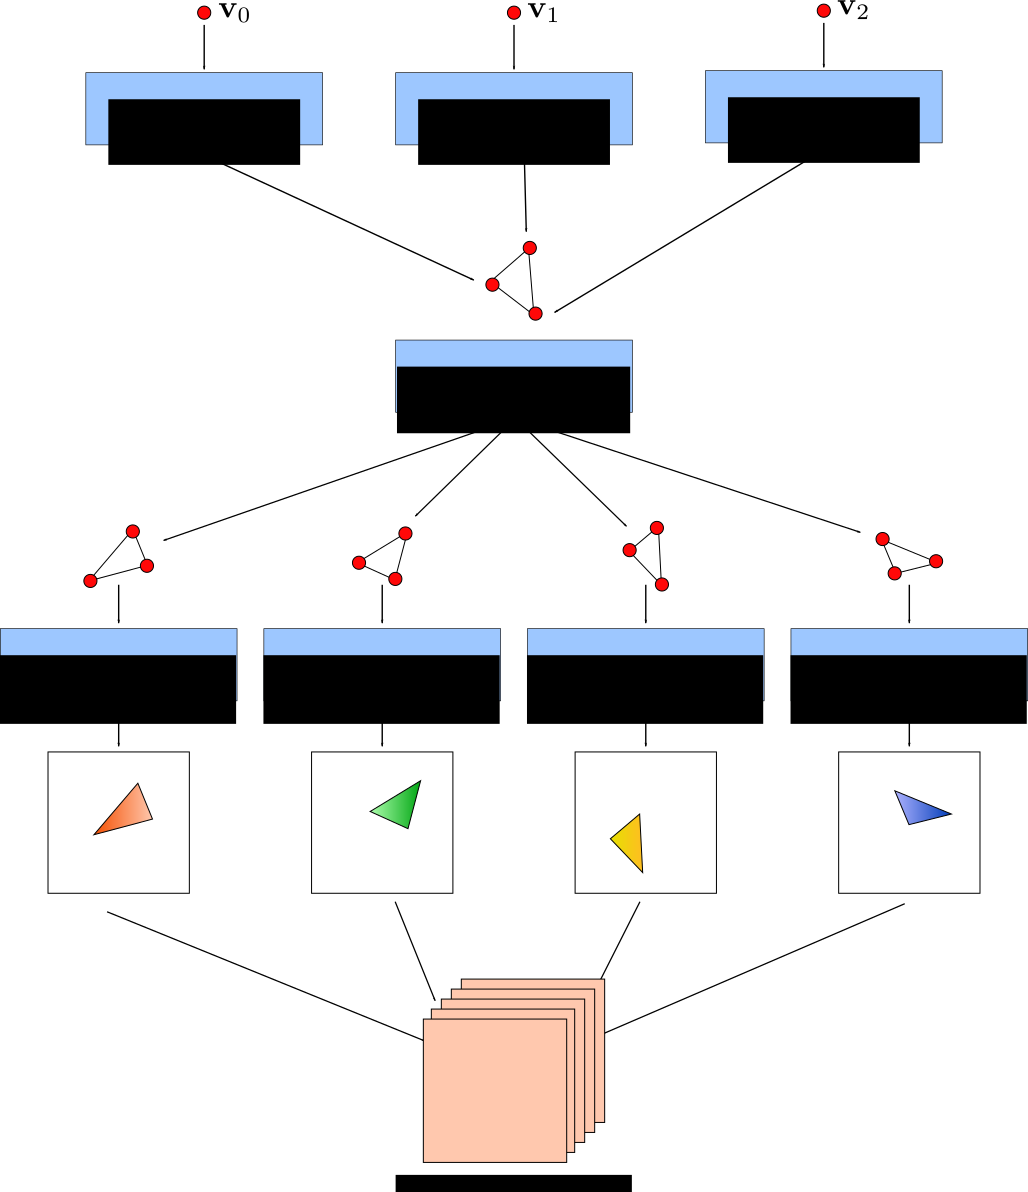
\includegraphics[width=\linewidth]{images/method/layered.pdf}
\caption{Diagram that illustrates layered rendering.}
\label{fig:step3}
\end{figure} 

We will use the OpenGL provided type \gl{GL_TEXTURE_2D_ARRAY}, that we initialize in the usual way, noting that an array texture should be initialized as a 3D texture. When binding it to an FBO, we use the generic \gl{glBindFramebufferTexture}:

\begin{lstlisting}[language=C++,label=lst:initarraytexture,caption={Initializing array texture. Note that the number of layers is passed to the \gl{glTexStorage3D} command.}]
GLuint fbo, arraytex;
glGenFramebuffers(1,&fbo);
glGenTextures(1, &arraytex);

glBindTexture(GL_TEXTURE_2D_ARRAY, arraytex);
[...] // setting up texture parameters, omitted
glTexStorage3D(GL_TEXTURE_2D_ARRAY, levels, GL_RGBA32F, size, size,layers);

glBindFramebuffer(GL_DRAW_FRAMEBUFFER, fbo);
glFramebufferTexture(GL_DRAW_FRAMEBUFFER, GL_COLOR_ATTACHMENT0, arraytex, 0);
\end{lstlisting}

In order to render to a layered texture, we need then to introduce a geometry shader. In our example, the difference between each layer is basically a different view matrix. So, we move the computation of the position, usually left to the vertex shader, to the geometry shader. We first introduce the code:

\begin{lstlisting}[language=GLSL,label=lst:arraygeomshader,caption={Geometry shader for layered rendering. The multiplication by the model matrix of vertex v is performed in the vertex shader (not shown).}]
#version 430
#define DIRECTIONS 16
layout(triangles) in;
layout(triangle_strip, max_vertices = 60) out;

uniform mat4 P;
uniform mat4 viewMatrices[DIRECTIONS];

void main(void)
{
    for(int i = 0; i < DIRECTIONS; i++)
    {
        gl_Layer = i;

        for(int k = 0; k < 3; k++)
        {
            vec4 v = gl_in[k].gl_Position;
            gl_Position = P * viewMatrices[i] * v;
            EmitVertex();
        }
        EndPrimitive();
    }
}
\end{lstlisting}

As we can see, we duplicate each one of the incoming triangles and then output it multiplied by a different view matrix. the \gl{EndPrimitive()} function ensures that the output triangles in the final triangle strip are separated. In order to render to a different layer each triangle, we need to set the special \gl{gl_Layer} variable to the layer we want to render before emitting the triangle. The whole process is illustrated in figure TODO.

\subsection{Accumulation buffers}

Often, during the rendering process, we would like to accumulate the result of a computation, in order to progressively update the result of the computation. In order to do this, we encounter an obstacle: we would like to render to the currently bound texture, but at the same time we need to read the previous value stored on the texture. Unfortunately, the OpenGL Specification \citep{openglspec} advices against reading from the same texture we are rendering to. This is made to avoid a situation called \emph{feedback loop}. In fact, we cannot be sure of the results of what is stored in any pixel of the texture while we are rendering to it. 

There are many possible solutions to the problem. The first approach is to rely on the driver implementation: some drivers, in fact, allow to render to the same texture we are bound to, under some conditions. However, if we want a general method that works over all platforms, we need not to rely on a implementation-dependent feature. The second solution is to use Image Textures. Image textures are a new type introduced in OpenGL 4.2 that allow explicit load-store of values, as well as new special constructs for GPU memory management (atomic operations and memory barriers). Though the usage of these features is appealing, their performance is generally poor compared to a framebuffer-based implementation. 

The final approach, and the one we describe in this chapter, is to use a technique called ping-pong. The idea is to sacrifice memory space by employing two textures $T_1$ and $T_2$. In the first frame, we render to the first texture $T_1$. IN the second frame, we use $T_2$ as a render target, and we sample $T_1$ and add it to the computed result. In the third frame, we render to $T_1$ and sample from $T_2$, and so on. From this alternance between the textures comes the name ping-pong. A minimal example of ping-ponging using a 2D texture is shown in listing \ref{lst:pingpong}.

\begin{lstlisting}[language=C++,label=lst:pingpong,caption={Minimal example of ping-pong textures.}]
// A global frame variable is initialized in order to keep track of the current frame

GLuint fbo, tex1, tex2;
// Creating FBO, initializing textures and texture parameters.
// Also binding shader with glUseProgram in order to bind texture uniforms
[...]

GLuint tex_from, tex_to;

tex_from = (frame % 2 == 0)? tex1 : tex2;
tex_to = (frame % 2 == 0)? tex2 : tex1;

glBindFramebuffer(GL_DRAW_FRAMEBUFFER, fbo);
glFramebufferTexture(GL_DRAW_FRAMEBUFFER, GL_COLOR_ATTACHMENT0, tex_to, 0);
glDrawBuffer(GL_COLOR_ATTACHMENT0);

GLint location = glGetUniformLocation("source_texture");
glUniform1i(location, 0);
glActiveTexture(GL_TEXTURE0);
glBindTexture(GL_TEXTURE_2D, tex_from);

// more uniforms and rendering commands.
[...]

frame ++;
\end{lstlisting}

\subsection{Generation of uniformly distributed points}
In our method we have at least twice the necessity to generate uniformly distributed points either on a disc or on a sphere. To do this, we employ a particular sequence of pseudo-random numbers, called \emph{Halton points} \citep{Halton:1964:ARQ:355588.365104}. We explain briefly the ideas behind the sequence. For a more mathematical complete discussion on its properties of pseudo randomness, see \cite{niederreiter1992a}. 

First, given a prime number $p$ and a nonnegative integer $n$, we can express it in base $p$ as:
$$
n = a_0 + {a_1} p + a_2 p^2 + ... + a_r p^r
$$  

Where $a_i \in [0, p - 1]$. We now define a van der Corput sequence $\Phi_p(n)$ as:

$$
\Phi_p(n) = \sum_{i = 0}^r \frac{a_i}{p^{i+1}} = \frac{a_0}{p} + ... + \frac{a_r}{p^r}
$$

This sequence, given te fact that is based on prime points, automatically assumes good qualities of randomness. In addition, the function is already normalized in the range $[0,1)$. We define an Halton point as the combination of two Van der Corput sequences:

$$
H_{p_1,p_2}(n) = (\Phi_{p_1}(n), \Phi_{p_2}(n))
$$ 

Where $p_1$ and $p_2$ are two prime numbers, with $p_1 < p_2$. Usually, $(p_1,p_2) = (2,3)$ gives good results. All Halton points belong to the region of space $[0,1]\times[0,1]$. In order to obtain a sampling of Halton points on a sphere, we convert them using an area-preserving cartesian-to-spherical coordinates formula:

\begin{equation*}
\begin{split}
&H_{p_1,p_2}(n) = (\Phi_{p_1}(n), \Phi_{p_2}(n)) \rightarrow (s,t) \Rightarrow \\
&\Rightarrow H^{sphere}_{p_1,p_2}(n) = (\sqrt{1 - (2t - 1) ^2} \cos(2\pi s),\sqrt{1 - (2t - 1) ^2} \sin(2\pi s), 2t-1) 
\end{split}
\end{equation*}

And, to get the point on a disc, we simply take the point on a sphere and project it. In practice, we put the third coordinate to zero:

\begin{equation*}
\begin{split}
&H_{p_1,p_2}(n) = (\Phi_{p_1}(n), \Phi_{p_2}(n)) \rightarrow (s,t) \Rightarrow\\
& \Rightarrow H^{disc}_{p_1,p_2}(n) = (\sqrt{1 - (2t - 1) ^2} \cos(2\pi s),\sqrt{1 - (2t - 1) ^2} \sin(2\pi s)) 
\end{split}
\end{equation*}

\cite{journals/jgtools/WongLH97} provide an introduction to Halton points, as well as describing an implementation to generate a point on a Van der Corput sequence. We implemented their pseudo-code in C++ as follows:

\begin{lstlisting}[language=C++,label=lst:vandercorput,caption={Generating the p-adic Van der Corput point.}]
float vanDerCorputPoint(int n, int basis)
{
    int kp = n;
    float pp = (float)basis;
    float phi = 0.0f;
    while(kp > 0)
    {
        int a = kp % basis;
        phi = phi + a / pp;
        kp = int(kp / basis);
        pp = pp * basis;
    }
    return phi;
}
\end{lstlisting}

\subsubsection{Exponentially biased points}
In our algorithm, in order to obtain a better sampling, we need to have an exponentially biased distribution of points, as described in section TODO in the method chapter. To obtain this disc, we employ a technique called rejection sampling. The general idea is to generate a the sequence of halton points, then calculate their radius $r$ and calculate its probability distribution function using a coefficient $\sigma_{tr}$. Then, we use the following acceptance criterion:

$$
e^{-\sigma_{tr} r} > \zeta
$$

Where $\zeta \in [0,1)$ is a pseudo-randomly generated number. We can see that if the point is close to the center ($r \rightarrow 0$), $e^{-\sigma_{tr} r} \approx 1$ and so the point is more probable to be accepted. On the other hand, if the point is far from the center of the disc ($r \rightarrow +\infty$), $e^{-\sigma_{tr} r} \approx 0$ and so the point is less probable to be accepted. The code for generating a vector of accepted points is reported in listing \ref{lst:randomexp}.

\begin{lstlisting}[language=C++,label=lst:randomexp,caption={Generation by rejection of a exponentially distributed disc.}]
void planeHaltonCircleRejectionExponential(std::vector<Vec2f> &result, int n, float sigma_tr)
{
    //Better method based on hemisphere
   unsigned int accepted = 0;
   unsigned int i = 1;
	
   while(accepted < n)
   {
        Vec2f point = haltonPointCircle(i, 2, 3);
        float radius = point.length();
        float expon = exp(-sigma_tr * radius);
        float zeta = rand() / ((float)(RAND_MAX));
        if(zeta < expon)
        {
            result.push_back(point);
            accepted++;
        }
        i++;
   }
}
\end{lstlisting}

\subsection{Shadow mapping}
Shadow mapping is a common technique used in modern real-time graphics \citep{everitt,Segal:1992:FSL:142920.134071,williams1978a}. The idea behind it is to render an object from a light's point of view, and then use the generated depth information in order to decide if a point is shadowed or not. First of all, we convert the point into the light camera space, using a special space conversion matrix. After this, if we have a point $\mathbf{p} = (p_x,p_y,p_z)$, we compare $p_z$ to the texture $T$ sampled in the point $(p_x,p_y)$:

$$
p_z < T(p_x,p_y)
$$ 

If the above condition is verified, it means that the current point is beneath the point visible from the light and then it should be shadowed. The matrix $L$ used to convert a point from world space to texture space is the following, using the matrix definitions and notation in section \ref{sec:matrices}:

$$
L = T\left(\frac{1}{2}\right) \cdot S\left(\frac{1}{2}\right) \cdot P \cdot V
$$

where $P$ and $V$ are the projection and view matrix we use to render with the light. The first two matrices are necessary to convert between clip and texture coordinates, as clip coordinates are in the range $[-1,1] \times [-1,1]$, while texture coordinates are in the range $[0,1]\times[0,1]$. The process is illustrated in figure TODO.

In our algorithm, we use the ideas behind shadow mapping in two different occasions. The first is to get the points $x_i$ in step 2 from the texture generated in step 1, where we use the matrix $L$ in order to convert the world point $\x_o$, corresponding to the pixel we are rendering to, into $\x_d$ the center of the disc in texture space. 

The second occasion is in the final combination step, where we use also shadow mapping in order to compute the visibility function $V^k(\x)$. Technically, the "light cameras` in this case are the directional cameras from where we render the scene, but the ideas behind are the same. We can see how we sample the shadow map in the final combination shader in the following listing:

\begin{lstlisting}[language=GLSL,label=lst:textureconfshadow,caption={Sampling of the shadow map texture in step 3 of our method.}]
#version 430
uniform sampler2DArrayShadow depthMap;
uniform mat4 cameraMatrices[DIRECTIONS];

float sample_shadow_map(vec3 world_pos, int layer)
{
		vec4 light_pos = cameraMatrices[layer] * vec4(world_pos,1.0f);
    light_pos.z -= shadow_bias; //bias to avoid shadow acne
    if(light_pos.x < 0.0 || light_pos.x > 1.0) return 1.0;
    if(light_pos.y < 0.0 || light_pos.y > 1.0) return 1.0;
    return texture(depthMap,vec4(light_pos.x,light_pos.y,layer,light_pos.z)).r;
}        
[...] //shader code
\end{lstlisting}

In the above code, \gl{cameraMatrices[layer]} corresponds to the $L$ matrix. The special type of sampler \gl{sampler2DArrayShadow}, is a special sampler type that makes something more than its equivalent \gl{sampler2DArray}. The latter, in fact, accepts a \gl{vec3}, and simply retrieves the value in the texture. The former, on the other hand, accepts an extra parameter $z_{camera}$ (which is \gl{light_pos.z}), and compares it to the value stored in the depth texture $z_{tex}$, performing the test in equation \ref{eq:shadowtest}. If the depth of the point is less than the depth stored in the texture ($z_{camera} < z_{tex}$), 1 is returned as the point is closer to the directional camera, and thus visible. On the other hand, if $z_{camera} \ge z_{tex}$, it means the point is under the surface, and thus not visible, and 0 is returned.

To configure the \gl{sampler2DArrayShadow} texture, we need to specify some extra parameters during the depth texture initialization:

\begin{lstlisting}[language=C++,label=lst:textureconfshadow,caption={Configuration of a shadow map depth texture.}]
glBindTexture(GL_TEXTURE_2D_ARRAY, depthtex);
glTexParameterf(GL_TEXTURE_2D_ARRAY, GL_TEXTURE_MIN_FILTER, GL_NEAREST);
glTexParameterf(GL_TEXTURE_2D_ARRAY, GL_TEXTURE_MAG_FILTER, GL_NEAREST);
glTexParameterf(GL_TEXTURE_2D_ARRAY, GL_TEXTURE_WRAP_S, GL_CLAMP_TO_EDGE);
glTexParameterf(GL_TEXTURE_2D_ARRAY, GL_TEXTURE_WRAP_T, GL_CLAMP_TO_EDGE);
glTexParameterf(GL_TEXTURE_2D_ARRAY, GL_TEXTURE_COMPARE_MODE, GL_COMPARE_REF_TO_TEXTURE);
glTexParameterf(GL_TEXTURE_2D_ARRAY, GL_TEXTURE_COMPARE_FUNC, GL_LESS);
glTexStorage3D(	GL_TEXTURE_2D_ARRAY, 1, GL_DEPTH_COMPONENT32F, size, size, layers);
\end{lstlisting}

We can see that we specify two extra parameters: \gl{GL_TEXTURE_COMPARE_MODE}, once set to \gl{GL_COMPARE_REF_TO_TEXTURE}, means that sampling the depth texture in a shader will give a value based on the comparison between an extra value $z$ and the depth value $d$ in the texture. The second parameter \gl{GL_TEXTURE_COMPARE_FUNC} specifies how to compare the values: \gl{GL_LESS} means that 1 is returned if $z<d$, and zero is returned otherwise. 

\section{Caveats}
The algorithm described so far, if implemented \emph{as is}, unfortunately does not give a result that we can appreciate. In order to obtain the desired result, some extra corrections are necessary.

\subsection{Random rotation of samples}
As we note in equation TODO, we never specified how the points in the samples are processed before actually being used in the calculation. This can lead to the assumption that the same disc pattern is used on every pixel. This causes a problem because this tends to generate banding artifacts, as we can see in figure TODO. In order to avoid the artifacts, in exchange for noise, is to randomly rotate the pattern per pixel. Given that we are able to generate a random point $r$, we can take each one of the samples on the disk $\mathbf{d}_i$ and rotate it in order to obtain the new sample $\mathbf{d}_i^*$:

\renewcommand{\arraystretch}{1}
\begin{equation}
\begin{split}
\theta &= 2 \pi r \\
\mathbf{d}_i^* &= \left(\begin{array}{cc}
\cos\theta & \sin\theta \\
-\sin\theta & \cos\theta \\
\end{array} \right) \ \mathbf{d}_i
\end{split}
\label{eq:randomrot}
\end{equation}
\renewcommand{\arraystretch}{1.8}

We can see the result in figure TODO. Even if noisy, this result does not have any artifacts. We will see how to reduce the noise using mip maps in section TODO. As we observed before in the overview, we also need the result to evolve on a time basis, in order not to compute the same results on every frame. Recalling that the current frame is $t$ and the maximum amount of frames before we stop the computations is $T$, we make our computation evolve using the following $\theta_t$ in equation \ref{eq:randomrot}:

$$
\theta_t = 2 \pi \left(r + \frac{t}{T}\right)
$$

This causes a progressive rotation of the disc around the point over time. However, we need still to specify how to calculate $r$. As a function, $r = (x,y,l)$ needs to depend on the fragment coordinates $(x,y)$, as well as from the current layer $l$ (to avoid two layers make the same computation). Since we are on the GPU, we cannot use a built-in random function, so we need either to load the random points from the CPU as a separate texture or to generate them on-the-fly. For the latter technique, we tried a sine based generator, with code on listing TODO, and a congruential linear generator in listing TODO. The input point that was given was in both cases $(l \cdot x, l \cdot y)$. We can see some results in figure TODO. The sine based generator gives the best result at the price of added computation time.

\begin{lstlisting}[language=GLSL,label=lst:sinegenerator,caption={Sine-based generation of random points on the GPU.}]
highp float noise(vec2 co)
{
    highp float a = 12.9898;
    highp float b = 78.233;
    highp float c = 43758.5453;
    highp float dt = dot(co.xy,vec2(a,b));
    highp float sn = mod(dt,3.14);
    return fract(sin(sn) * c);
}
\end{lstlisting}


\begin{lstlisting}[language=GLSL,label=lst:lineargenerator,caption={Linear Congruential generator of random points on the GPU.}]
highp float noise(vec2 co)
{
    return (co.x + 2048.0f * co.y) * 3125.0f + 49.0f;
}
\end{lstlisting}

\subsection{Mipmap generation}
The randomization we performed in the previous step comes with a drawback, i.e. we increase the noisiness of the result, especially in the initial steps. Once we reach convergence, the noisiness slowly disappears, as we can see from figure TODO. In order to improve our method, we need to introduce a way to take the intermediate result and make it as close as possible to the final result at convergence. Our approach was to use a filter to blur the result multiple times, storing the results in the mipmaps of the radiance map generated in step 2 of our method. This results in an additional step between step 2 and step 3, where the mip maps are calculated.

We tried different filters with different weights, and we will test some of them in the result chapter. The one that gave us the most promising results is the bilinear filter with the shape shown in figure TODO. The filter uses the alpha value of the texture as a weight for the sampled color, so the filter maintain the edges of the texture. We can see in figure TODO a comparison between the standard mipmap filter (which is an averaging of four neighbouring pixels) and our bilinear filter, noticing immediately the result.

On the implementation level, the mipmaps need to be rendered one after the other, as we need the result of the first computation in order to perform the second. So, we use always the same shader, reported in listing \ref{lst:shaderimageprocessing}, to filter between two textures. In the first step, we bind layer zero (where the result of the rendering of step 2 is stored) as source and layer one as destination. Then, we bind layer 1 as source and layer 2 as destination, and so on. To perform the filtering, we render a full screen quad.

However, OpenGL natively does not allow to bind the same image both as a source and as a destination, even if the mipmap levels are different. So, in order to overcome this difficulty, we use a new OpenGL feature called \emph{texture views}. Texture views are a way to create a texture in OpenGL, but on the opposite hand of \gl{glTexImage*D} or the \gl{glTexStorage*D} families of functions they allow to use another texture storage as the storage point for the current texture. The name comes from the fact that we can use texture views to see the content of a texture from two different points of view, by interpreting the storage in two different ways. In our case, we create a new texture for the mipmaps, but then we configure it to use the storage reserved to the mipmaps of the radiance map. So, we can bind it to the FBOS as it was a completely different texture, but then once we render the result will be rendered exactly where we want. Figure TODO offer a visual explanation.

\begin{lstlisting}[language=GLSL,label=lst:shaderimageprocessing,caption={Custom mipmap filtering on GPU. \gl{_tex} are the texture coordinates on the screen aligned quad.}]
#version 430
in vec3 _tex;
uniform sampler2DArray source;

out vec4 fragColor;

uniform float texStep;
uniform int scaling;

void main(void)
{
	int layer = gl_Layer;
	float t_step = texStep * 0.5 * scaling;
	vec4 c0  = texture(source,vec3(_tex.xy,layer));
	vec4 c1  = texture(source,vec3(_tex.xy + vec2(t_step,0.0f),layer));
	vec4 c2  = texture(source,vec3(_tex.xy - vec2(t_step,0.0f),layer));
	vec4 c3  = texture(source,vec3(_tex.xy + vec2(0.0f, t_step),layer));
	vec4 c4  = texture(source,vec3(_tex.xy - vec2(0.0f, t_step),layer));

	vec4 c5  = texture(source,vec3(_tex.xy + 2 * vec2(t_step,0.0f),layer));
	vec4 c6  = texture(source,vec3(_tex.xy - 2 * vec2(t_step,0.0f),layer));
	vec4 c7  = texture(source,vec3(_tex.xy + 2 * vec2(0.0f, t_step),layer));
	vec4 c8  = texture(source,vec3(_tex.xy - 2 * vec2(0.0f, t_step),layer));

	vec4 c9  = texture(source,vec3(_tex.xy + vec2(t_step,t_step),layer));
	vec4 c10 = texture(source,vec3(_tex.xy - vec2(t_step,t_step),layer));
	vec4 c11 = texture(source,vec3(_tex.xy + vec2(t_step, -t_step),layer));
	vec4 c12 = texture(source,vec3(_tex.xy - vec2(t_step, -t_step),layer));

	float v0 = clamp(c0.a,0.0f,1.0f);
	float v1 = clamp(c1.a,0.0f,1.0f);
	[...] //omitted
	float v12 = clamp(c12.a,0.0f,1.0f);

	vec4 step1 = c0 * v0 + c1 * v1 + c2 * v2 + c3 * v3 + c4 * v4;
	float vstep1 = v0 + v1 + v2 + v3 + v4;
	vec4 step2 = c5 * v5 + c6 * v6 + c7* v7 + c8 * v8;
	float vstep2 = v5 + v6 + v7 + v8;
	vec4 step3 = c9 * v9 + c10 * v10 + c11 * v11 + c12 * v12;
	float vstep3 = v9 + v10 + v11 + v12;

	fragColor = (step1 + step2 + step3 )/max(vstep1 + vstep2 + vstep3, 1.0f);
}
\end{lstlisting}
\subsection{Shadow bias}
The shadow mapping described in section TODO has an obvious problem, called \emph{shadow acne}. As we can see in figure TODO, the discretization of depth comes with a problem: depending on the incidence angle, the surface starts generating an alternating pattern of dark and light on the visible areas. The solution in this case is to introduce a constant factor when we are comparing the texture space position and the depth of a point, called \emph{shadow bias} $\epsilon_b$. The test then becomes:

$$
p_z - \epsilon_b < T(p_x,p_y)
$$ 

The result is depicted in figure TODO. As we can see, we raise the sampling by the bias factor, so the lit areas do not present shadow acne anymore. This comes with a drawback: the shadow bias, for thin objects, it introduces another artifact, called \emph{peter panning}, i.e. the shadow and the object become disconnected. In the case of our method, a too large bias makes the different directions to become "disconnected`, not representing a faithful result. 

\subsection{Texture discretization artifacts}
A problem related to the previous one is texture discretization artifacts, that appear as seams in the texture in figure TODO. The problem is similar to the one of depth bias, but it manifests on the direction perpendicular to the directional cameras. Because of the discretization and the depth bias in the shadow sampling, some pixels become false positives, being incorrectly sampled even if they are not visible. To fix this, we apply a transformation to the vertex in the final step that shrinks it a little bit towards the center of the texture. The shrinking is made using the camera direction as a main axis, according to the formula:

$$
\x_o^{shrink} = \x_o - \epsilon_c (\vec{n}_o - \vomega_d (\vec{n}_o \cdot \vomega_d));
$$

Where $\epsilon_c = \frac{1}{W}$, where $W$ is the width of the radiance map in pixel. In this way we obtain a shrinkage of one pixel of the model when we use $\x_o^{shrink}$ for sampling the radiance map. As we can see in figure TODO, adding this correction solves the problem.

\chapter{Results}
\label{chap:results}
In this chapter, after we discussed the implementation of our method, we are going to check it after the assumptions we stated in chapter \ref{chap:intro}, discussing advantages, disadvantages, and trade-offs that was necessary to account for. In the first section, we will discuss the quality result of our method, comparing it to path-traced results. In the second section, we will discuss how close we can get to the expected results in the performance domain, seeing how well our implementation scales in different domains. 

\section{Parameters}
\label{sec:parameters}
In this section, we are going to refer to some parameters of our method. The parameters were introduced in the previous chapter \ref{chap:implementation}. We will sum them up here, in order to have a reference for this chapter.

\begin{itemize}
\item $M$, the total number of points in the disk. We recall that we make a disc of the size of the object bounding box and then generate $M$ exponentially based samples in it. Unless otherwise stated, $M = 1000$
\item $q$, the modifier of the exponential distribution of the samples. So, the points are distributed on a circle with PDF $q \sigma_{tr}\exp(-q\sigma_{tr} r)$. Unless otherwise stated, $q = 1$. We choose $\sigma_{tr} = min(\sigma_{tr, red},\sigma_{tr, green},\sigma_{tr, blue})$, i.e. the minimum component spectrum wise.
\item $N$, the number of samples used from the disc. It is always $N < M$.
\item $K$, the number of directions used in the radiance map. Unless otherwise stated, $K = 16$. 
\item $L$, the number of lights in the scene. 
\item $W_l$, the size in pixel of the lightmaps. Unless otherwise stated, $W_l = 512$.
\item $W_r$, the size in pixel of the radiance map. Unless otherwise stated, $W_r = 1024$.
\end{itemize}


Other parameters are available in the method, such as all the parameters of the cameras. But even if we did not, those can be set up automatically. In this section, we listed only the parameters that makes sense for the user to tweak, and that can directly influence the quality or the performance of the final result.

\section{Quality comparison}

In the domain of quality, we compared our method to a solution obtain with a Monte Carlo path tracer that uses the directional dipole. The solutions are compared only visually, since if was not possible to perfectly match the perspective and view cameras of the original pictures. Thus, a RMSE comparison would not make sense.  We will see that the visual results of our method, given enough samples, can produce a result ofter comparable to the one of a path traced solution. We will compare our results at convergence (after 100 frames of evolution), to then also compare some of the results obtained during the evolution of the method. 

\subsection{Tests with different number of samples}

The material tested where potato, a highly scattering isotropic material ($\alpha = \sigma_s / \sigma_a \approx 10^2$), a even higher high scattering material, marble ($\alpha \approx 10^4$), a material with a big forward scattering component, white grapefruit juice ($\alpha \approx 10^2$, $g \approx 0.5$), ketchup a material that has a strong absorption component in the red channel ($\alpha_{red} \approx 10^{-2}$, $\alpha_{green} \approx \alpha_{blue} \approx 10^2$), and beer, a high absorption, forward scattering material with nearly no scattering. We are biased against highly scattering material because those are the material where our BSSRDF model gives our best results. However, we included materials as beer and ketchup to provide a comparison of our method even where the orgiginal BSSRDF model should fail.

The first comparison we make is with the path traced spheres generated in figure \ref{fig:examplesmaterials}. The results are illustrated in figure \ref{fig:pathpotato}, comparing different values of $M$ and $N$ for a potato sphere. We can see that different values of $M$ and $N$ greatly influence the results. In fact, for a big $M$ and the same $N$, the samples tend to be closer to the exitance point $x_o$, so the results is more accurate on the highlight region. If instead we chose a relatively small $M$, the points are more spread on the surface, to the absorption of the material is accounted more. This result in a sphere with gradients that are closer to the path trace solution. In this case, the highlights are way more difficult to see. 

The result that gets closer to the path traced solution is the one where $N = M = 1000$, but as we will see this values are unfeasible in the realm of performance, even for simple models. So, it is the artist that should find the right balance between $M$ and $N$ in order to get a satisfying result. 

In all cases, however, we observe a color shift to a greenish material compared to the path traced solution. Our guess is that the radius we are using is based on the minimum transmission coefficient $\sigma_{tr}$, that for potato is $\sigma_tr \approx (7, 14, 49) dm^{-1}$. So, the absorption is accounted more for the channels with the highest transmission coefficients (in this case, green and blue), that is probably causing the color shift. We will see that for materials with more homogenous scattering and absorption coefficients this phenomena is way more limited (as for example, in grapefruit juice and marble in figures  \ref{fig:pathgrapefruit} and \ref{fig:pathmarble}).

\begin{figure}
\centering
\subfloat[{$N = 120$, $M = 120$}]{
  \includegraphics[width=0.33 \linewidth]{images/results/test_120_over_120.png}
}
\subfloat[{$N = 120$, $M = 300$}]{
  \includegraphics[width=0.33 \linewidth]{images/results/test_120_over_300.png}
}
\subfloat[{$N = 300$, $M = 300$}]{
  \includegraphics[width=0.33 \linewidth]{images/results/test_300_over_300.png}
} \\
\subfloat[{$N = 120$, $M = 1000$}]{
  \includegraphics[width=0.33 \linewidth]{images/results/test_120_over_1000.png}
}
\subfloat[{$N = 300$, $M = 1000$}]{
  \includegraphics[width=0.33 \linewidth]{images/results/test_300_over_1000.png}
}
\subfloat[{$N = 1000$, $M = 1000$}]{
  \includegraphics[width=0.33 \linewidth]{images/results/test_1000_over_1000.png}
} \\
\subfloat[Path traced solution]{
  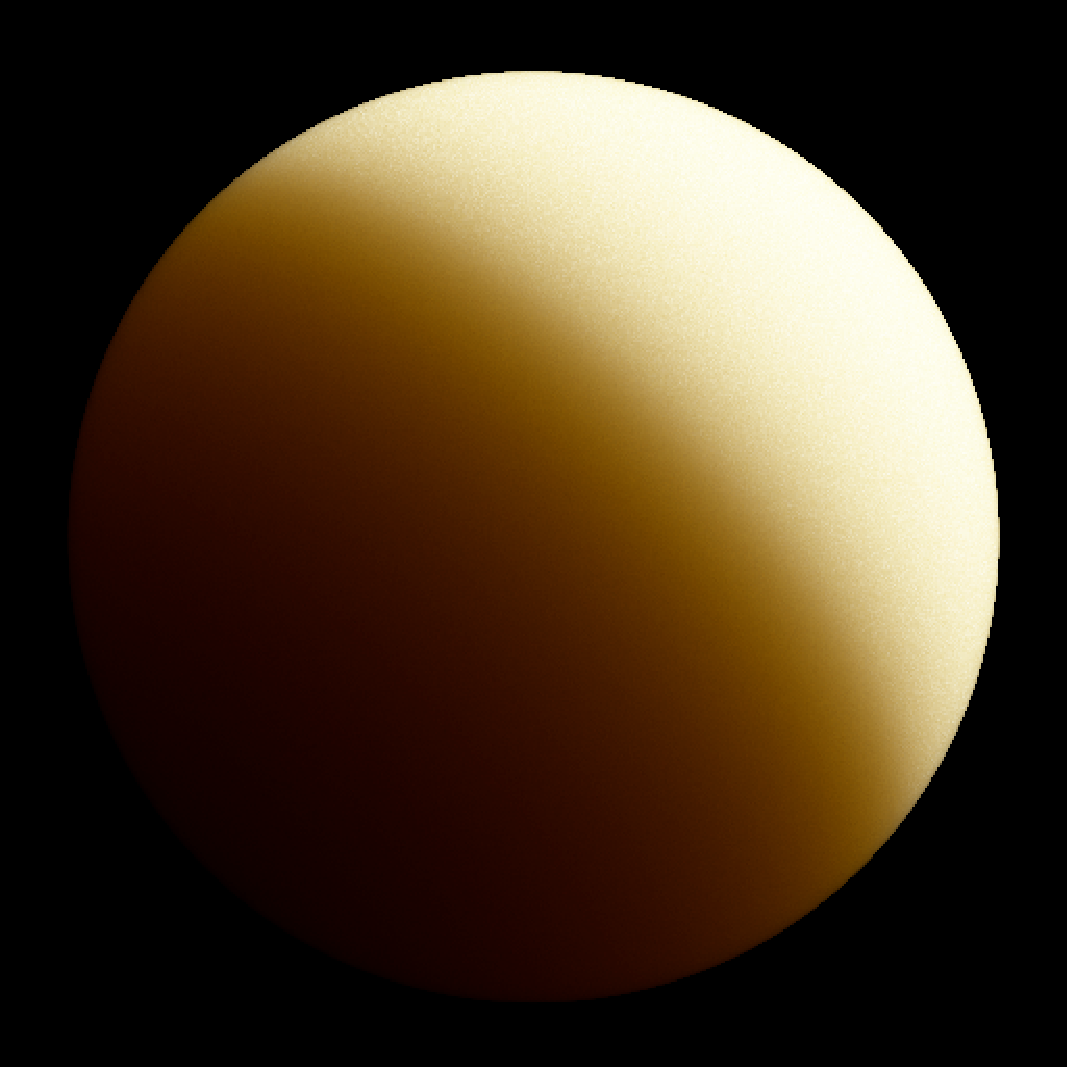
\includegraphics[width=0.33 \linewidth]{images/pathtrace/image-potato.pdf}
}
 \\
\caption{Path traced rendering on a sphere of potato material compared with the results of our method. The parameters are from table \ref{table:scatteringcoefficients}.}
\label{fig:pathpotato}
\end{figure}
 
In the next set of experiments, we can see the utility of the $q$ parameter. We tested a sphere of white grapefruit juice in figure \ref{fig:pathgrapefruit}, a material with a high forward scattering component. In this case we can see that that with a smaller number of samples $N = 100$ and a $q = 3$ we can approximate very well the solution where $N = 1000$ and $q = 1$, way more expensive for the GPU. In a test with marble, in figure \ref{fig:pathmarble} we can see that our sampling introduces artifacts, especially on the color transition area. In this case, $q$ slightly relieves the artifacts generated from the sampling. Also in this case, our method does not capture the red color shift of the path traced solution, due to a higher blue scattering coefficient.

\begin{figure}
\centering
\subfloat[{$N = 100$, $M = 1000$, $q = 1$}]{
  \includegraphics[width=0.5 \linewidth]{images/results/grapefruit_juice_comparison_100_over_1000_nobias.png}
}
\subfloat[{$N = 100$, $M = 1000$, $q = 3$}]{
  \includegraphics[width=0.5 \linewidth]{images/results/grapefruit_juice_comparison_100_over_1000_bias3.png}
}
\\
\subfloat[{$N = 1000$, $M = 1000$, $q = 1$}]{
  \includegraphics[width=0.5 \linewidth]{images/results/grapefruit_juice_comparison.png}
}
\subfloat[{Path traced result}]{
  \includegraphics[width=0.5 \linewidth]{images/pathtrace/image-grapefruit.pdf}
}
\caption{Path traced rendering on a sphere of white grapefruit material compared with the results of our method. The parameters are from table \ref{table:scatteringcoefficients}. We can see that a higher $q$ helps us in approximating the path traced solution with fewer samples.}
\label{fig:pathgrapefruit}
\end{figure}

\begin{figure}
\centering
\subfloat[{$N = 120$, $M = 1000$, $q = 1.5$}]{
  \includegraphics[width=0.4 \linewidth]{images/results/marble_120_over_1000_bias_1-5.png}
}
\subfloat[{$N = 120$, $M = 1000$, $q = 1$}]{
  \includegraphics[width=0.4 \linewidth]{images/results/marble_120_over_1000_nobias.png}
}
\\
\subfloat[{$N = 1000$, $M = 1000$, $q = 1.5$}]{
  \includegraphics[width=0.4 \linewidth]{images/results/marble_1000_over_1000_bias_2.png}
}
\subfloat[{$N = 1000$, $M = 1000$, $q = 1$}]{
  \includegraphics[width=0.4 \linewidth]{images/results/marble_1000_over_1000_biasno.png}
}
\\
\subfloat[{Path traced result}]{
  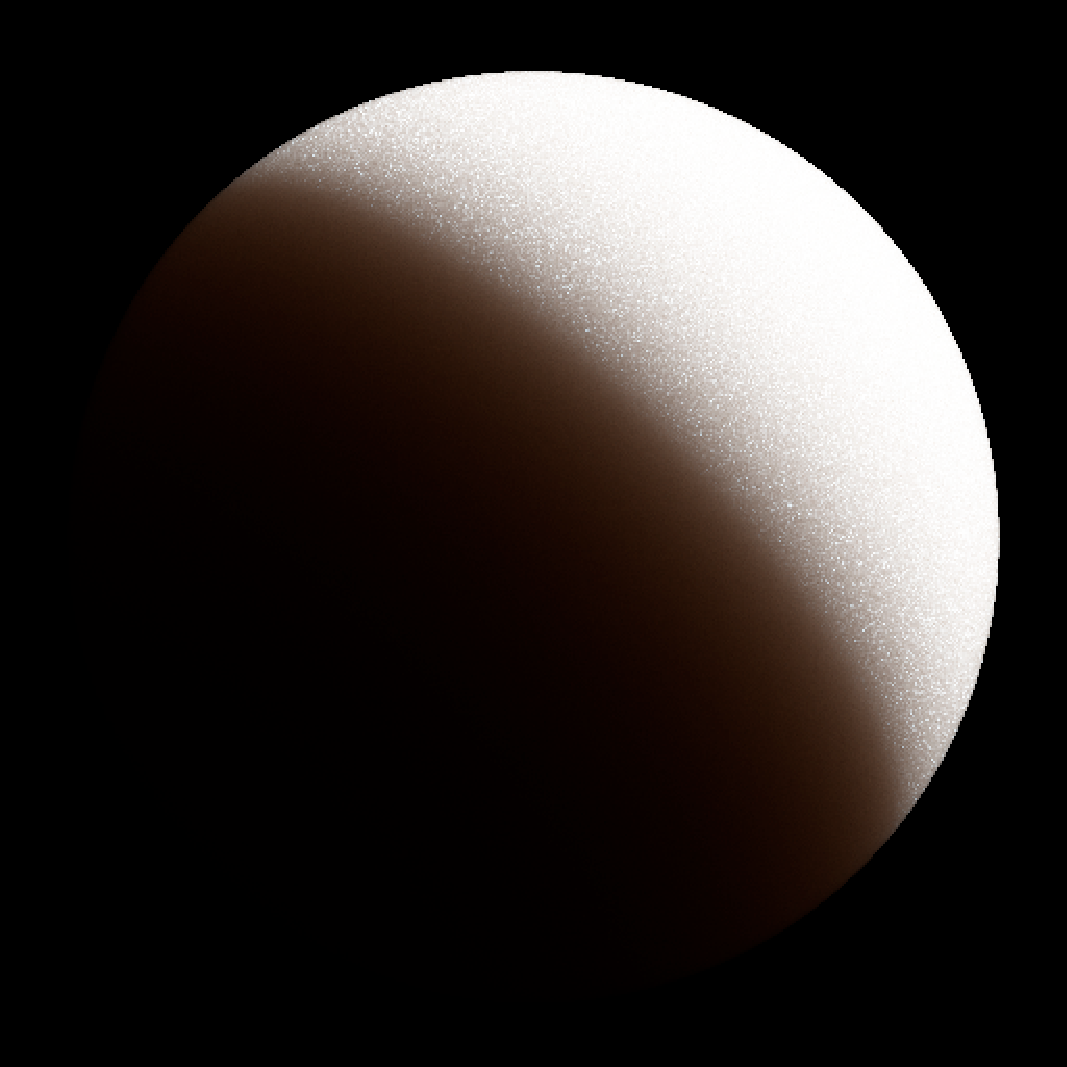
\includegraphics[width=0.4 \linewidth]{images/pathtrace/image-marble.pdf}
}
\caption{Path traced rendering on a sphere of marble material compared with the results of our method. The parameters are from table \ref{table:scatteringcoefficients}.}
\label{fig:pathmarble}
\end{figure}

\FloatBarrier
In figure \ref{fig:pathbeer}, we can see a comparison between our method and a beer material: despite the obvious artifacts due to sampling, our results show a more realistic result that a path traced one. This happens because of the extremely low scattering coefficient of beer, that makes it unfeasible to use a Monte Carlo path tracer, since we need to sum a lot of contribution in order to remove all the noise. 

\begin{figure}[!ht]
\centering
\subfloat[{$N = 100$, $M = 100$, $q = 1$}]{
  \includegraphics[width=0.5 \linewidth]{images/results/beer_100_over_100_no_bias.png}
}
\subfloat[{Path traced result}]{
  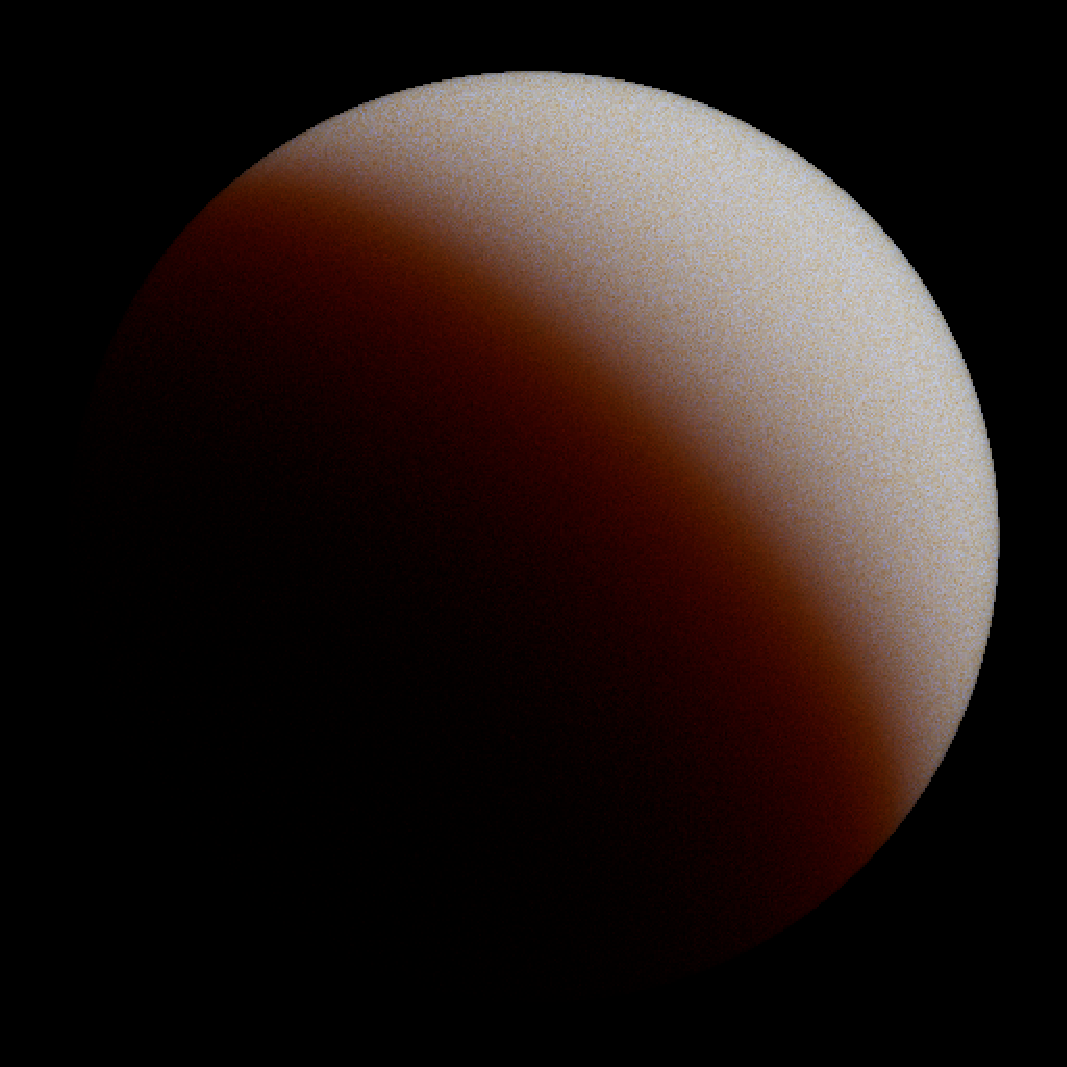
\includegraphics[width=0.5 \linewidth]{images/pathtrace/image-beer.pdf}
}
\caption{Path traced rendering on a sphere of beer material compared with the results of our method. The parameters are from table \ref{table:scatteringcoefficients}.}
\label{fig:pathbeer}
\end{figure}

The results that we obtained in the sphere renderings affect also the rendering of the full models. We tested a buddha made of potato and a dragon made of ketchup, that will be tested for performance in section \ref{sec:perf}. For the buddha, we observe a similar result (color shift) compared to reference as for the spheres in figure \ref{fig:pathpotato}.

For the ketchup dragon, instead, we observe that for a very low number of concentrated samples, the absorption contribution disappears, leaving only a gray scattering contribution that exhibits a pearling effect. If we reduce $M$, the highlights reduce and the absorption of the red part of the spectrum is accounted for.


\begin{figure}
\centering
\subfloat[{$N = 100$, $M = 1000$, $q = 1$}]{
  \includegraphics[width=0.333 \linewidth]{images/results/happy_buddha_100_over_1000_nobias.png}
}
\subfloat[{$N = 200$, $M = 1000$, $q = 1$}]{
  \includegraphics[width=0.333 \linewidth]{images/results/happy_buddha_200_over_1000_nobias.png}
}
\\
\subfloat[{$N = 100$, $M = 300$, $q = 1$}]{
  \includegraphics[width=0.333 \linewidth]{images/results/happy_buddha_100_over_300_nobias.png}
}
\subfloat[{Path traced result}]{
  \includegraphics[width=0.333 \linewidth]{images/results/potato_buddha_dir.png}
}
\caption{Rendering of a potato buddha using the directional dipole, with increasing number of samples.}
\label{fig:pathbuddha}
\end{figure}


\begin{figure}
\centering
\subfloat[{$N = 10$, $M = 100$, $q = 1.5$}]{
  \includegraphics[width=0.5 \linewidth]{images/results/dragon_10_over_100.png}
}
\subfloat[{$N = 50$, $M = 120$, $q = 1$}]{
  \includegraphics[width=0.5 \linewidth]{images/results/dragon_50_over_120.png}
}
\\
\subfloat[{$N = 50$, $M = 1000$, $q = 1.5$}]{
  \includegraphics[width=0.5 \linewidth]{images/results/dragon_50_over_1000_nobias.png}
}
\subfloat[{Path traced result}]{
  \includegraphics[width=0.5 \linewidth]{images/results/ketchup_dragon_dir.png}
}
\label{fig:pathdragon}
\caption{Rendering of a ketchup dragon using the directional dipole, with changing values of $M$ and $N$. }
\end{figure}

\clearpage
\subsection{Radiance map sizes tests}
Finally, we tested the effect of reducing the size of the texture used for the radiance map, for the dragon test. As we can see, for diminishing values of $W_s$ the quality does not get too much worse until $W_s = 128$, where artifacts due to shadow mapping become evident. In figure \ref{fig:pathdragonsizett} the difference between the 1024 and the 256 image is reported. In the image, we can see that most of the difference are within $10\%$ of the high resolution value (since the image is enlarged 10 times and the full colored pixels are only a minority).

\begin{figure}[!h]
\centering
  \includegraphics[width=0.7 \linewidth]{images/results/difference.png}
\caption{Difference multiplied by 10 times between \ref{fig:pathdragonsize1024} and \ref{fig:pathdragonsize256}.}
\label{fig:pathdragonsizett}
\end{figure}

\begin{figure}
\centering
\subfloat[{$W_s = 128$}]{
  \includegraphics[width=0.5 \linewidth]{images/results/dragon_50_over_120_ws128.png}
}
\subfloat[{$W_s = 256$}]{
  \includegraphics[width=0.5 \linewidth]{images/results/dragon_50_over_120_ws256.png}
	\label{fig:pathdragonsize256}
}
\\
\subfloat[{$W_s = 512$}]{
  \includegraphics[width=0.5 \linewidth]{images/results/dragon_50_over_120_ws512.png}
	\label{fig:pathdragonsize512}
}
\subfloat[{$W_s = 1024$}]{
  \includegraphics[width=0.5 \linewidth]{images/results/dragon_50_over_120_detail.png}
	\label{fig:pathdragonsize1024}
}
\label{fig:pathdragonsize}
\caption{Rendering of a ketchup dragon using the directional dipole, with varying radiance map size $W_s$.}
\end{figure}

\FloatBarrier
\subsection{Tests of mipmap blurring quality}

In this part we tested the quality improvement from the mipmap blurring introduced in section \ref{sec:mipmaps} to the final image. We can see the result of our method at the first frame of our simulation for different mipmap levels. At the beginning of the evolution, a strong blurring (two passes) is needed to compensate the high level noise, as we can see from image \ref{fig:mipblurring}. During the evolution, a lesser level of mipmaps is needed in order to preserve a noiseless image. At convergence, we do not need mipmap blurring at all, as the result converge to the solution. 
\begin{figure}[!h]
\vspace{-0.5cm}
\centering
\subfloat[{Mipmap level 0 (no blur)}]{
  \includegraphics[width=0.4 \linewidth]{images/results/mipmaps00.png}
}
\subfloat[{Mipmap level 1}]{
  \includegraphics[width=0.4 \linewidth]{images/results/mipmaps01.png}
} \\

\subfloat[{Mipmap level 2}]{
  \includegraphics[width=0.4 \linewidth]{images/results/mipmaps02.png}
}
\subfloat[{Convergence}]{
  \includegraphics[width=0.4 \linewidth]{images/results/mipmapsc.png}
}

\caption{Detail of rendering of a potato dragon in the first frame of the computation for different mipmap levels. We can see that the second mipmap level is very close to the final result. However, some artifacts due to the stretching of the mipmap appear, such as black spots and bright seams. All the figures use $N = 32$ and $M = 300$.}
\label{fig:mipblurring}
\end{figure}
\FloatBarrier

\subsection{Environment map illumination}

All the given consideration so far are the same irregardless if we have an environment map or a single directional light. In this section we present the results obtained we environment light illumination. Visually, we obtain a nice result. Obviously, since the samples are split between different lights, an overlapping is inevitable, and we need an higher number of samples to obtain a decent result. The bunny in figure \ref{fig:bunnyenv1} was obtained using 16 directional lights, sampled using the method in \ref{sec:envenv} and \ref{sec:env}, with $N = 80$ (5 samples per light) and $M = 1000$. 

As for reference, we compared our results to the reference image of the potato buddha from \cite{IMM2013-06646} in figure \ref{fig:pathbuddhaenv}. We had to try to match the light settings and the camera, but here as well we notice the same color shift as before. Also in this case we used 16 directional lights to represent our skybox.

\begin{figure}[!h]
\centering
\includegraphics[width=0.7 \linewidth]{images/results/bunny_env_80_1000_nobias.png}
\caption{Marble Bunny rendered in the Doge environment map. Note that the light is predominantly from the up direction.}
\label{fig:bunnyenv1}
\end{figure}

%\begin{figure}
%\centering
%\subfloat[{Grace Cathedral}]{
%  \includegraphics[width=0.5 \linewidth]{images/results/bunny_envgrace_80_1000_nobias.png}
%}
%\subfloat[{Pisa Courtyard}]{
%  \includegraphics[width=0.5 \linewidth]{images/results/bunny_envPISA_80_1000_nobias.png}
%}
%\caption{Marble bunny rendered in two other environment maps, Grace Catherdal and Pisa Courtyard.}
%\label{fig:bunnyenv}
%\end{figure}


\begin{figure}
\centering
\subfloat[{$L = 16$, $N = 90$, $M = 1000$}]{
  \includegraphics[width=0.333 \linewidth]{images/results/happy_buddha_environment_90over16_1000_nobias.png}
}
\subfloat[{$L = 16$, $N = 90$, $M = 320$}]{
  \includegraphics[width=0.333 \linewidth]{images/results/happy_buddha_environment_90over16_310_nobias.png}
}
\\
\subfloat[{$L = 16$, $N = 90$, $M = 160$}]{
  \includegraphics[width=0.333 \linewidth]{images/results/happy_buddha_environment_90over16_160_nobias.png}
}
\subfloat[{Path traced result}]{
  \includegraphics[width=0.333 \linewidth]{images/results/reference_env.png}
}
\caption{Rendering of a potato buddha using our environment lighting and the Doge map.}
\label{fig:pathbuddhaenv}
\end{figure}

\clearpage
In the image of figure \ref{fig:dragonenv}, we compare the result using the Pisa Courtyard environment map on a Stanford Dragon, comparing a different number of lights. We can see the more lights we introduce, the more closer we get to a result that approximate true environment illumination. We observe also that the images have more scattering than absorption the more we increase the number of lights: this is because the total number of samples $N$ does not change, so each light has less and less samples available. In this way, the samples tend to concentrate in the center and produce a result where the scattering component is predominant.
\begin{figure}[!h]
\vspace{-0.5cm}
\centering
\subfloat[{2 lights}]{
  \includegraphics[width=0.4 \linewidth]{images/results/env2.png}
}
\subfloat[{4 lights}]{
  \includegraphics[width=0.4 \linewidth]{images/results/env4.png}
} \\

\subfloat[{8 lights}]{
  \includegraphics[width=0.4 \linewidth]{images/results/env8.png}
}
\subfloat[{16 lights}]{
  \includegraphics[width=0.4 \linewidth]{images/results/env16.png}
}
\caption{Rendering of a potato dragon ($N = 32$, $M = 300$) using a different number of directional light to represent the environment map.}
\label{fig:dragonenv}
\end{figure}

\clearpage
\section{Performance tests}
\label{sec:perf}
In this section, we examine and analyze the performance of our method. The tests in this section were made by keeping in mind the performance requirements we made in chapter \ref{chap:intro}, and they exploit how the different parameters listed in \ref{sec:parameters} influence the final result. For the tests, we used three main models, to which we will refer as Bunny, Dragon and Buddha (see table \ref{table:models}). The models cover a varying range of complexity. The Bunny model represents a typical model used in modern games and consoles ($10^4$ triangles), while the Dragon represents a highly detailed model, usually for visualization purposes ($10^5$ triangles). Finally, the Buddha model represent a high resolution model, and it will be used as a stress test for our algorithm ($10^6$ triangles).

\begin{table}[!ht]
\centering
\begin{tabular}{|l|l|l|}
\hline
Model  & Vertices (\#$V$) & Triangles (\#$\Delta$) \\ \hline
Bunny  & $3581$                                   & $21474 \approx 10^4$                           \\ \hline
Dragon & $50000$                                  & $300000 \approx 10^5$                          \\ \hline
Buddha & $549409$                                 & $3262422 \approx 10^6$                         \\ \hline
\end{tabular}
\caption{The three models used for our tests, with number of vertices and triangles.}
\label{table:models}
\end{table}

All the tests were performed on a NVIDIA GeForce GTX 780Ti, a high-end modern GPU with OpenGL 4.3 capabilities. All the timings measure the average milliseconds during the 20th and the 40th frame during an evolution to convergence of 100 frames. The first frames were not measured because of the overhead introduced by the initialization procedure (texture creation, model parsing and loading, shader compilation, etc.).

\subsection{Time algorithm breakdown}

The first test we are going to perform is to time how much time the algorithm takes to perform the different steps illustrated in chapter \ref{chap:implementation}. When we were timing the algorithm, we divided the whole computation into five different steps:

\begin{enumerate}
	\item Initialization phase, where all the different constants and data structures in the algorithm are created and initialized.
	\item Render to light map step, that corresponds to step 1 in our outline.
	\item Render to radiance map step, that corresponds to step 2 in our outline.
	\item Mipmap generation, as in the extension outlined in section \ref{sec:mipmaps}.
	\item Final render combination, that corresponds to step 3 in our outline.
\end{enumerate}

For this tests we tried all the three models, and the results are shown in figure \ref{fig:timingssplit}. The parameters were tweaked in order to reach the best compromise between visual quality and performance, in order to measure realistic timings. 

We can observe that, irregardless of the test case, most of the time is spent computing the BSSRDF function for the samples in step 2. Thee render to lightmap step does not have a big performance impact, likely because all the tests were made with one light. We will test in the next section the impact of a different number of lights on the performance.  Another consideration to do is that, as to be expected, the more triangles we have the less samples we can use. As we will see, this is not the only factor that causes a performance drop. However, the big number of triangles that has to be multiplied by the number of directions generates a big load on the GPU for rasterization procedures. 

Regarding the mipmap generation, as expected its performance is not tied to the size of the model, but only to the size of the radiance map texture $W_l$ and to the number of mipmaps we generate. Finally, the final combination step is tied as well to the size of the model, rising slightly with an increasing model size. However, in this case we are rendering only once the model to the main framebuffer, and not $K$ times as in step 2.

\begin{figure}
\centering
\subfloat[Beer Bunny, $67.6 ms$. Point light. $N = 180$, $M = 210$, $q = 2$]{
  \includegraphics[width=0.4 \linewidth]{images/results/example2.png}
}
\subfloat[Detailed timings.]{
\begin{tabular}[b]{lllll}
\multicolumn{5}{c}{\includegraphics[width=0.3 \linewidth]{images/matlab/bunnychart.pdf}}                                                   \\ \hline
\multicolumn{1}{|l|}{RL}   & \multicolumn{1}{l|}{RR}    & \multicolumn{1}{l|}{MG}   & \multicolumn{1}{l|}{FR}   & \multicolumn{1}{l|}{Tot}   \\ \hline
\multicolumn{1}{|l|}{0.36} & \multicolumn{1}{l|}{65.18} & \multicolumn{1}{l|}{1.03} & \multicolumn{1}{l|}{1.00} & \multicolumn{1}{l|}{67.57} \\ \hline
\end{tabular}
}\\
\subfloat[Ketchup Dragon, $60.3 ms$. Directional light. $N = 20$, $M = 180$.]{
  \includegraphics[width=0.4 \linewidth]{images/results/example1.png}
}
\subfloat[Detailed timings.]{
\begin{tabular}[b]{lllll}
\multicolumn{5}{c}{\includegraphics[width=0.3 \linewidth]{images/matlab/dragonchart.pdf}}                                                   \\ \hline
\multicolumn{1}{|l|}{RL}   & \multicolumn{1}{l|}{RR}    & \multicolumn{1}{l|}{MG}   & \multicolumn{1}{l|}{FR}   & \multicolumn{1}{l|}{Tot}   \\ \hline
\multicolumn{1}{|l|}{1.13} & \multicolumn{1}{l|}{55.93} & \multicolumn{1}{l|}{0.97} & \multicolumn{1}{l|}{2.21} & \multicolumn{1}{l|}{60.25} \\ \hline
\end{tabular}
}\\
\subfloat[Potato Buddha, $92.9 ms$. Point light. $N = 10$, $M = 300$, $q = 1$]{
  \includegraphics[width=0.4 \linewidth]{images/results/example3.png}
}
\subfloat[Detailed timings.]{
\begin{tabular}[b]{lllll}
\multicolumn{5}{c}{\includegraphics[width=0.3 \linewidth]{images/matlab/buddhachart.pdf}}                                                   \\ \hline
\multicolumn{1}{|l|}{RL}   & \multicolumn{1}{l|}{RR}    & \multicolumn{1}{l|}{MG}   & \multicolumn{1}{l|}{FR}   & \multicolumn{1}{l|}{Tot}   \\ \hline
\multicolumn{1}{|l|}{10.27} & \multicolumn{1}{l|}{79.30} & \multicolumn{1}{l|}{0.88} & \multicolumn{1}{l|}{2.48} & \multicolumn{1}{l|}{92.93} \\ \hline
\end{tabular}
}
\caption{Rendering of different models, and graphs that illustrate how the timings are split into the different phases of the algorithm. All tests use $W_l = W_s = 512$. The acronyms represent RL = Render to lightmap, RR = Render to radiance map, MG = Mipmap Generation and FR = Final Rendering.}
\label{fig:timingssplit}
\end{figure}

\FloatBarrier
\subsection{Tests for varying parameters}
In this section, we will discuss how well our method behaves for changing parameters. From the quality tests before we have learned that the parameters that are related mostly to the quality of the are $N$, $M$, $q$ and to a certain extent $W_s$. The number of directions $K$ is important in order to ensure to cover the whole model, and if we are generating the cameras automatically it cannot be too low. Of the mentioned parameters, $M$ and $q$ do not directly influence performance, as they are used only at the beginning of the computation in order to distribute the points on the disc. 
 
\textbf{$N$ parameter}\\
We start by discussing $N$. We can see the results for different value of the parameter in the following table:

\begin{table}[!ht]
\centering
\begin{tabular}{p{3cm}l|l|l|l|l|}
\cline{3-6}
                             &      & \multicolumn{4}{c|}{Number of samples ($N$)}                                          \\ \cline{3-6} 
Model                        & \#$\Delta$& \multicolumn{1}{c|}{1} & \multicolumn{1}{c|}{10} & \multicolumn{1}{c|}{50} & \multicolumn{1}{c|}{100} \\ \hline
\multicolumn{1}{|l|}{Bunny}  & $10^4$ & \mycolor{4}.1                  & \mycolor{10}.1                 & \mycolor{21}.4                  & \mycolor{38}.7                 \\ \hline
\multicolumn{1}{|l|}{Dragon} & $10^5$ & \mycolor{13}.9                 & \mycolor{35}.2                  & \mycolor{139}.6                & \mycolor{270}.8                \\ \hline
\multicolumn{1}{|l|}{Buddha} & $10^6$ & \mycolor{91}.5                 & \mycolor{93}.0                  & \mycolor{121}.4                & \mycolor{209}.2                 \\ \hline
\end{tabular}
\caption{Timings in milliseconds of our method for different models and number of samples $N$ (potato material properties). The other parameters were $L = 1$, $W_s = W_l = 512$, $M = 1000$, $K = 16$.}
\end{table}

We tested $N$ in the range $1-100$. The test with $N = 1$ was introduced to measure the baseline performance of the method (where the most expensive operation is the generation of the random number for the rotation). We did not use zero samples because otherwise the shader compiler optimizations would have removed the base code as well, making the result useless.

We note that from the graph the time to render the dragon with 50 samples is slower that rendering the buddha with the same parameters, despite the buddha having 10 times the triangles as the dragon. This suggests that $N$ and the triangle size of the model are not the only factors involved in the performance. Since the heavy computational step is made on a pixel shader in step 2, the number of pixels involved in the computation matters: the buddha on average occupies less texture area on the directional cameras, and thus the number of computations performed in total is less that the ones for the dragon. For a low number of samples, the performance is bound by the rasterization time, so the dragon outperforms the buddha in this case because of the fewer number of triangles. 

We tested this changing performance according to the area in the following test: we kept the same settings for the directional cameras, but we tried different dragon sizes. By size, we mean the size of the dragon using a different scaling transform matrix.

\begin{table}[!ht]
\centering
\begin{tabular}{p{3cm}l|l|l|l|l|}
\cline{3-6}
                             &      & \multicolumn{4}{c|}{Size of the model (units)}                                          \\ \cline{3-6} 
Model                        & \#$\Delta$& \multicolumn{1}{c|}{1} & \multicolumn{1}{c|}{0.5} & \multicolumn{1}{c|}{0.25} & \multicolumn{1}{c|}{0.125} \\ \hline
\multicolumn{1}{|l|}{Dragon}  & $10^5$ & \mycolor{147}.3                  & \mycolor{73}.7                 & \mycolor{14}.1                  & \mycolor{11}.7                 \\ \hline
\end{tabular}
\caption{Timings in milliseconds of our method for different model size (potato material properties). The size of the camera is 2 units, and the model is 2 units wide. The camera does not scale with the model. The other parameters were $N = 50$, $L = 1$, $W_s = W_l = 512$, $M = 1000$, $K = 16$.}
\end{table}

The dragon, by changing size, occupies a different area of the camera, and so the algorithm performs differently according to the dragon size. A degrading in quality of the final result is also visible, because of the less number of pixels involved. This problem should be addressed in an eventual extension to the implementation, that should account for these problems in a optimal camera placement.

\textbf{$W_s$ parameter}\\
The next test we performed was on the size of the radiance map. 

\begin{table}[!ht]
\centering
\begin{tabular}{p{3cm}l|l|l|l|l|}
\cline{3-5}
                             &      & \multicolumn{3}{c|}{Size of the radiance map ($W_s$)}                                          \\ \cline{3-5} 
Model                        & \#$\Delta$& \multicolumn{1}{>{\centering\arraybackslash}p{1.2cm}|}{256} & \multicolumn{1}{>{\centering\arraybackslash}p{1.2cm}|}{512} & \multicolumn{1}{>{\centering\arraybackslash}p{1.2cm}|}{1024} \\ \hline
\multicolumn{1}{|l|}{Bunny}  & $10^4$ & \mycolor{12}.1                  & \mycolor{20}.2                 & \mycolor{40}.2                               \\ \hline
\multicolumn{1}{|l|}{Dragon} & $10^5$ & \mycolor{76}.0                 & \mycolor{139}.7                  & \mycolor{291}.1                             \\ \hline
\multicolumn{1}{|l|}{Buddha} & $10^6$ & \mycolor{92}.1                 & \mycolor{122}.1                  & \mycolor{252}.6                             \\ \hline
\end{tabular}
\caption{Timings in milliseconds of our method for different models and size of the radiance map $W_s$ (ketchup material properties). The other parameters were $N = 50$, $L = 1$, $W_l = 512$, $M = 1000$, $K = 16$.}
\label{table:sizews}
\end{table}

As we can see from table \ref{table:sizews}, the performance scales linearly with the radiance map size. This means that if we double the size of the radiance map, the time to render the model roughly doubles. This comes from the fact that most of the time in the computation is spent in rendering to the radiance map, that is a pixel bound operation. So if we double the size of map, we roughly double the number of pixels involved and thus the number of the fragment shader invocations in step 2. 

\textbf{$K$ parameter}\\
The next test is about the number of directions used to render the model, $K$.

\begin{table}[!ht]
\centering
\begin{tabular}{p{3cm}l|l|l|l|l|}
\cline{3-6}
                             &      & \multicolumn{4}{c|}{Number of directions ($K$)}                                          \\ \cline{3-6} 
Model                        & \#$\Delta$& \multicolumn{1}{c|}{4} & \multicolumn{1}{c|}{8} & \multicolumn{1}{c|}{16} & \multicolumn{1}{c|}{32} \\ \hline
\multicolumn{1}{|l|}{Bunny}  & $10^4$ & \mycolor{6}.3                  & \mycolor{15}.0                 & \mycolor{22}.8                  & \mycolor{44}.0                 \\ \hline
\multicolumn{1}{|l|}{Dragon} & $10^5$ & \mycolor{37}.9                 & \mycolor{68}.1                  & \mycolor{141}.0                & \mycolor{299}.4                \\ \hline
\multicolumn{1}{|l|}{Buddha} & $10^6$ & \mycolor{29}.9                 & \mycolor{54}.8                  & \mycolor{120}.4                & \mycolor{327}.0                 \\ \hline
\end{tabular}
\caption{Timings in milliseconds of our method for different models and different number of directions $K$ (ketchup material properties). The other parameters were $N = 50$, $L = 1$, $W_s = W_l = 512$, $M = 1000$, $q = 1$.}
\end{table}

We can see that the performance for the models scales linearly. We can see from this test that is a big advantage to place the cameras manually, instead of relying on an automatic algorithm. A careful placement of the cameras can cover the whole model evenly with a smaller number of cameras that an automatic placement. In our implementation, we needed to use at least 16 cameras to ensure that most of the models were covered. On the other hand, with careful placement of the cameras, we were able to lower the number of cameras up to 8 in all cases, thus doubling the performance. Also in this test, we can see that the minor area occupation of the buddha improves its performance for 4,8, and 16 directions. For 32 directions, the number of triangles that actually need to be rasterized ($32 \cdot 10^6$) probably becomes so high that memory issues on the GPU become important.

\textbf{Different types of lights}\\
We tested the different times in performance for different kind of lights. Since the operations performed are roughly the same (the point light requires an extra division), also is the performance:

\begin{table}[!ht]
\centering
\begin{tabular}{p{3cm}l|l|l|l|}
\cline{3-5}
                             &      & \multicolumn{3}{c|}{Type of light}                                          \\ \cline{3-5} 
Model                        & \#$\Delta$& \multicolumn{1}{c|}{Point light} & \multicolumn{1}{c|}{Directional light}  & \multicolumn{1}{c|}{No loop} \\ \hline
\multicolumn{1}{|l|}{Dragon}  & $10^5$ & \mycolor{60}.5                  & \mycolor{60}.3                            & \mycolor{58}.2                 \\ \hline
\end{tabular}
\caption{Timings in milliseconds of our method for different types of light (potato material properties), one light. The other parameters were $N = 20$, $W_s = W_l = 512$, $M = 1000$, $K = 16$.}
\end{table}

We times a third case, that is when we strip the outer loop in listing \ref{lst:multi}, thus obtaining a shader suitable for only one light. In this case, we can see that the performance slightly improves by 2 milliseconds.

\textbf{Different materials}\\
We finally tried to see if different materials gave a different performance on the method. As we expected, the material does not influence the rendering time, as the computations in the BSSRDF do not actually take advantage on the material type to easy any computation. We can see the test result in the following table:
\begin{table}[!ht]
\centering
\begin{tabular}{p{3cm}l|l|l|l|l|}
\cline{3-6}
                             &      & \multicolumn{4}{c|}{Material}                                          \\ \cline{3-6} 
Model                        & \#$\Delta$& \multicolumn{1}{c|}{Ketchup} & \multicolumn{1}{c|}{Beer} & \multicolumn{1}{c|}{White grapefruit} & \multicolumn{1}{c|}{Potato} \\ \hline
\multicolumn{1}{|l|}{Dragon}  & $10^5$ & \mycolor{87}.7                  & \mycolor{86}.6                 & \mycolor{87}.6                 & \mycolor{88}.4                 \\ \hline
\end{tabular}
\caption{Timings in milliseconds of our method for different materials. The other parameters were $N = 30$, $L = 1$, $W_s = W_l = 512$, $M = 300$, $K = 16$.}
\end{table}

\clearpage
\subsection{Tests on environment lighting}
The considerations so far discussed apply also in environment map lighting, that we converted to a certain number $L$ of directional lights. So discussing the impact on performance of multiple lights and the impact of environment lighting is essentially the same, apart from a initialization delay to generate the lights from the environment map that we will not consider.

The timings for different kind of lights are reported in the following table:
\begin{table}[!ht]
\centering
\begin{tabular}{p{3cm}l|l|l|l|l|l|}
\cline{3-7}
                             &                      & \multicolumn{5}{c|}{Number of lights $L$}                                                             \\ \cline{3-7} 
Model                        & \#$\Delta$ & \multicolumn{1}{c|}{1} & \multicolumn{1}{c|}{2} & \multicolumn{1}{c|}{4} & \multicolumn{1}{c|}{8} &  \multicolumn{1}{c|}{16} \\ \hline
\multicolumn{1}{|l|}{Dragon}  & $10^5$ & \mycolor{91}.1                 & \mycolor{95}.9                 & \mycolor{96}.4                 & \mycolor{101}.5            & \mycolor{108}.1      \\ \hline
\end{tabular}
\caption{Timings in milliseconds of our method for different number of lights (environment map approximation, material properties for potato). The other parameters were $N = 32$, $W_s = W_l = 512$, $M = 300$, $K = 16$.}
\label{table:multilightenvdragon}
\end{table}
\vspace{-0.2cm}
As we can see, even if we maintain the same number of samples ($N = 32$, so the number of samples per light changes) the performance worsen increasing the number of lights. To look at this into more detail, we broke down the timings again in the different steps. We can see in figure \ref{fig:numblights} that the increase in timing is due to step 1, the render to lightmap: in fact, we have to render the model once for each light, that implies a performance penalty.

\begin{figure}[!ht]
\centering
  \includegraphics[width=0.7\linewidth]{images/matlab/multiple_lights_test.pdf}

\caption{Rendering times for the environment lighting of figure \ref{table:multilightenvdragon}, split into the various components. The rendering times of step 2 are not shown, but they are $[87.2\ 90.2\ 89.4\ 91.6\ 95.2]$.}
\label{fig:numblights}
\end{figure}

\chapter{Future work}
\label{chap:futurework}

In this chapter we discuss the improvements that can be done to our method in order to improve the solution.

\section{Improving the quality}

As we have seen the results section, catching the right effect balancing absorption and scattering requires a lot of tweaking of the parameters $M$ and $q$. This depends from the fact that an exponential sampling based on $\sigma_{tr}$ is not probably the best suited for the solution, thus providing good results. A further investigation of optimal sampling patterns would be required in order to obtain faithful results.

An idea we would like to explore is to use two separate disks with a different sampling radius, one accounting the absorption and one for the scattering contribution. The size of the radius of the two disk should be related to the scattering parameters, such as $\sigma_a$ and $\sigma_s$. Further investigation is required in this realm in order to obtain results applicable to a wide range of participating media.

Another direction we would like to explore is the automatic placing of the cameras. Because of the variety and possible concavity of meshes, it is very difficult to place cameras in a way to ensure the complete coverage of the object. The field in which to find ideas in order to fully cover the object would be 3D mesh acquisition using cameras. In this way, it will be possible for a user to avoid the tedious operation of placing the cameras in order to get a full coverage of the object. 

Another possibility in this area is to rotate the cameras during the rendering phase: in this case, fewer cameras will be necessary, but then an accumulation process would not be possible in the way we implemented it. It would require a great change to the way the algorithm works in order to get a solution.

\section{Improving the performance}
Regarding the implementation, we tought about some possible extensions in order to make the implementation faster and more reliable.

The first thing we have thought about would be to change the loop in step 2. The idea would be to have instead to have a single fragment shader invocation with cycling $N$ times on the samples, to have $N$ separate fragment shader invocations that calculate the result. The single invocations can be summed over using blending or atomic operations available since OpenGL 4.2. This would allow the GPU more flexibility in scheduling its work. However, we have seen in TODO that also the random number generation is an expensive operation for the GPU, and that would have to be repeated for each of the $N$ fragments, potentially undermining the advantages of GPU scheduling. 

Another improvement in order to make the performance more reliable would be to make the cameras more adaptive. At the moment, the size of the light and directional cameras is fixed and set up by the user. A simple extension to the method would be to make the camera size adaptive, in order to adapt to the object bounding box. This would make the area in the radiance map texture space more consistent regarding to the size of the object, leading to a more predictable result. 


\chapter{Conclusions}
\label{chap:conclusions}

In this thesis, we have presented an approch to rendering translucent materials using a new directional subsurface scattering BSSRDF models. We focused on creating a method that renders translucent materials in real-time, thus approximating well path traced results.

In chapter \ref{chap:previous} we gave an overview of the different approaches to rendering subsurface scattering in literature, identifying the gap in the knowledge in rendering translucent materials efficiently using a directional approach.

In chapter \ref{chap:theory}, we instroduced the mathematical concepts that are needed to give a basic understanding of light transport theory and BSSRDF models, introducing the nthe formulation of two BSSRDF dipole models, the standard dipole model and the directional dipole model. Using this knowledge, we gave the reader a theoretical introduction to our method, as well as scattering parameters and how they are acquired in chapter \ref{chap:method}. Chapter \ref{chap:method} provided an essential bridge between theory and implementation, that we described in chapter \ref{chap:implementation}. In the implementation, we described a method that employs the advantages of the formulation of the directional dipole in order to create a robust method that implements the directional dipole taking advantage of the GPU rendering pipeline.

In chapter \ref{chap:results}, we compared our result to path traced solutions, proving that our method can produce results that approximate well path-traced solutions, providing speed ups of four order of magnitude compared to path tracing on CPU. We also proved that our method for models of the size commonly used in the computer game industry performs in real-time on a high-end modern GPU, limiting the size of memory used to a minimum. 

Finally, in chapter	\ref{chap:futurework}, we introduced some possible ideas to expand our method in order to produce a higher quality result retaining its real-time capabilities.

To sum up, we think that most of the goals of the thesis stated in the introduction chapter have been satisfied. This thesis hopefully provides an insight on a new way to approach the efficient rendering of translucent materials using directional subsurface scattering. 
\appendix
\chapter{Model matrices}
\label{sec:matrices}
\section{Model matrices}

\textbf{Translation matrix}

$$T(\mathbf{t}) = \left[\begin{array}{cccc}
1 & 0 & 0 & \mathbf{t}_x       \\
0 & 1 & 0 & \mathbf{t}_y       \\
0 & 0 & 1 & \mathbf{t}_z       \\
0 & 0 & 0 & 1
\end{array}\right]$$


\textbf{Rotation matrix}

$$R_x(\theta) = \left[\begin{array}{cccc}
1 & 0 & 0 & 0       \\
0 & \cos\theta & -\sin\theta & 0       \\
0 & \sin\theta & \cos\theta & 0      \\
0 & 0 & 0 & 1
\end{array}\right]$$

$$R_y(\theta) = \left[\begin{array}{cccc}
\cos\theta & 0 & \sin\theta & 0       \\
0 & 1 & 0 & 0       \\
-\sin\theta & 0 & \cos\theta & 0      \\
0 & 0 & 0 & 1
\end{array}\right]$$

$$R_z(\theta) = \left[\begin{array}{cccc}
\cos\theta & -\sin\theta & 0 & 0       \\
\sin\theta & \cos\theta & 0 & 0       \\
0 & 0 & 1 & 0      \\
0 & 0 & 0 & 1
\end{array}\right]$$

\textbf{Scale matrix}

$$S(\mathbf{s}) = \left[\begin{array}{cccc}
\mathbf{s}_x & 0 & 0 & 0       \\
0 & \mathbf{s}_y & 0 & 0       \\
0 & 0 & \mathbf{s}_z & 0      \\
0 & 0 & 0 & 1
\end{array}\right]$$

\section{View Matrix}

$\mathbf{e}$ is the camera position, $\mathbf{d}$ is the camera direction, $\mathbf{u}$ is the up vector.

\begin{equation*}
\begin{split}
\vec{c} &= -\frac{\mathbf{d}}{\|\mathbf{d}\|} \\
\vec{a} &= \frac{\vec{c} \times \mathbf{u}}{\|\vec{c} \times \mathbf{u}\|} \\
\vec{b} &= \vec{a} \times \vec{c} 
\end{split}
\end{equation*}

$$
V(\mathbf{e},\mathbf{d},\mathbf{u}) = \left[\begin{array}{cccc}
\vec{a}_x & \vec{a}_y & \vec{a}_z & -\mathbf{e}_x      \\
\vec{b}_x & \vec{b}_y & \vec{b}_z & -\mathbf{e}_y        \\
\vec{c}_x & \vec{c}_y & \vec{c}_z & -\mathbf{e}_z       \\
0 & 0 & 0 & 1
\end{array}\right]$$

\section{Projection Matrix}

\textbf{Orthographic matrix}

$\mathbf{l}$ is the left bottom near corner of the frustum, $\mathbf{r}$ is the top right far corner.

$$
O(\mathbf{l},\mathbf{r}) = \left[\begin{array}{cccc}
\frac{2}{\mathbf{r}_x-\mathbf{l}_x} & 0 & 0 & -\frac{\mathbf{r}_x+\mathbf{l}_x}{\mathbf{r}_x-\mathbf{l}_x}       \\
0 & \frac{2}{\mathbf{r}_y-\mathbf{l}_y} & 0 & -\frac{\mathbf{r}_y+\mathbf{l}_y}{\mathbf{r}_y-\mathbf{l}_y}      \\
0 & 0 &  - \frac{2}{\mathbf{r}_z-\mathbf{l}_z} & -\frac{\mathbf{r}_z+\mathbf{l}_z}{\mathbf{r}_z-\mathbf{l}_z}      \\
0 & 0 & 0 & 1
\end{array}\right]
$$

\textbf{Perspective matrix}

$fov$ is the field of view in radians, $A$ is the aspect ratio, $n_p$ is the near camera plane and $f_p$ is the far camera plane. We define:

$$
f_c = \frac{1}{\tan(\frac{fov}{2})}
$$

$$
P(fov,A,n,f) = \left[\begin{array}{cccc}
\frac{f_c}{A} & 0 & 0 & 0       \\
0 & f_c & 0 & 0       \\
0 & 0 & \frac{n + f}{n - f} & \frac{2 n f}{n-f}      \\
0 & 0 & -1 & 0
\end{array}\right]
$$


                                 %Appendix A
%-----------
% Backmatters

%-----------
\backmatter
\chaptermark{Bibliography}
\renewcommand{\sectionmark}[1]{\markright{#1}}
\sectionmark{Bibliography}
\addcontentsline{toc}{chapter}{Bibliography}        %Force addition of Bibliography to TOC
\bibliographystyle{alexnat}                           %Use alpha codes for references
\bibliography{thesis}                           %Bibliography file called
\end{document}